% Template for PLoS
% Version 3.6 Aug 2022
%
% % % % % % % % % % % % % % % % % % % % % %
%
% -- IMPORTANT NOTE
%
% This template contains comments intended
% to minimize problems and delays during our production
% process. Please follow the template instructions
% whenever possible.
%
% % % % % % % % % % % % % % % % % % % % % % %
%
% Once your paper is accepted for publication,
% PLEASE REMOVE ALL TRACKED CHANGES in this file
% and leave only the final text of your manuscript.
% PLOS recommends the use of latexdiff to track changes during review, as this will help to maintain a clean tex file.
% Visit https://www.ctan.org/pkg/latexdiff?lang=en for info or contact us at latex@plos.org.
%
%
% There are no restrictions on package use within the LaTeX files except that no packages listed in the template may be deleted.
%
% Please do not include colors or graphics in the text.
%
% The manuscript LaTeX source should be contained within a single file (do not use \input, \externaldocument, or similar commands).
%
% % % % % % % % % % % % % % % % % % % % % % %
%
% -- FIGURES AND TABLES
%
% Please include tables/figure captions directly after the paragraph where they are first cited in the text.
%
% DO NOT INCLUDE GRAPHICS IN YOUR MANUSCRIPT
% - Figures should be uploaded separately from your manuscript file.
% - Figures generated using LaTeX should be extracted and removed from the PDF before submission.
% - Figures containing multiple panels/subfigures must be combined into one image file before submission.
% For figure citations, please use "Fig" instead of "Figure".
% See http://journals.plos.org/plosone/s/figures for PLOS figure guidelines.
%
% Tables should be cell-based and may not contain:
% - spacing/line breaks within cells to alter layout or alignment
% - do not nest tabular environments (no tabular environments within tabular environments)
% - no graphics or colored text (cell background color/shading OK)
% See http://journals.plos.org/plosone/s/tables for table guidelines.
%
% For tables that exceed the width of the text column, use the adjustwidth environment as illustrated in the example table in text below.
%
% % % % % % % % % % % % % % % % % % % % % % % %
%
% -- EQUATIONS, MATH SYMBOLS, SUBSCRIPTS, AND SUPERSCRIPTS
%
% IMPORTANT
% Below are a few tips to help format your equations and other special characters according to our specifications. For more tips to help reduce the possibility of formatting errors during conversion, please see our LaTeX guidelines at http://journals.plos.org/plosone/s/latex
%
% For inline equations, please be sure to include all portions of an equation in the math environment.  For example, x$^2$ is incorrect; this should be formatted as $x^2$ (or $\mathrm{x}^2$ if the romanized font is desired).
%
% Do not include text that is not math in the math environment. For example, CO2 should be written as CO\textsubscript{2} instead of CO$_2$.
%
% Please add line breaks to long display equations when possible in order to fit size of the column.
%
% For inline equations, please do not include punctuation (commas, etc) within the math environment unless this is part of the equation.
%
% When adding superscript or subscripts outside of brackets/braces, please group using {}.  For example, change "[U(D,E,\gamma)]^2" to "{[U(D,E,\gamma)]}^2".
%
% Do not use \cal for caligraphic font.  Instead, use \mathcal{}
%
% % % % % % % % % % % % % % % % % % % % % % % %
%
% Please contact latex@plos.org with any questions.
%
% % % % % % % % % % % % % % % % % % % % % % % %

\documentclass[10pt,letterpaper]{article}
\usepackage[top=0.85in,left=2.75in,footskip=0.75in]{geometry}

% amsmath and amssymb packages, useful for mathematical formulas and symbols
\usepackage{amsmath,amssymb}

% Use adjustwidth environment to exceed column width (see example table in text)
\usepackage{changepage}

% textcomp package and marvosym package for additional characters
\usepackage{textcomp,marvosym}

% cite package, to clean up citations in the main text. Do not remove.
\usepackage{cite}

% Use nameref to cite supporting information files (see Supporting Information section for more info)
\usepackage{nameref,hyperref}

% line numbers
\usepackage[right]{lineno}

% ligatures disabled
\usepackage[nopatch=eqnum]{microtype}
\DisableLigatures[f]{encoding = *, family = * }

% color can be used to apply background shading to table cells only
\usepackage[table]{xcolor}

% array package and thick rules for tables
\usepackage{array}

% create "+" rule type for thick vertical lines
\newcolumntype{+}{!{\vrule width 2pt}}

% create \thickcline for thick horizontal lines of variable length
\newlength\savedwidth
\newcommand\thickcline[1]{%
  \noalign{\global\savedwidth\arrayrulewidth\global\arrayrulewidth 2pt}%
  \cline{#1}%
  \noalign{\vskip\arrayrulewidth}%
  \noalign{\global\arrayrulewidth\savedwidth}%
}

% \thickhline command for thick horizontal lines that span the table
\newcommand\thickhline{\noalign{\global\savedwidth\arrayrulewidth\global\arrayrulewidth 2pt}%
\hline
\noalign{\global\arrayrulewidth\savedwidth}}

% TODO: replace with thickhline commands above?
\usepackage{booktabs}

% Inline comments for authors by initials.
\def\jhc#1{\textcolor{red}{[#1]}}
\def\snc#1{\textcolor{blue}{[#1]}}

% Remove comment for double spacing
\usepackage{setspace}
\doublespacing

% Text layout
\raggedright
\setlength{\parindent}{0.5cm}
\textwidth 5.25in
\textheight 8.75in

% Bold the 'Figure #' in the caption and separate it from the title/caption with a period
% Captions will be left justified
\usepackage[aboveskip=1pt,labelfont=bf,labelsep=period,justification=raggedright,singlelinecheck=off]{caption}
\renewcommand{\figurename}{Fig}

% Use the PLoS provided BiBTeX style
\bibliographystyle{plos2015}

% Remove brackets from numbering in List of References
\makeatletter
\renewcommand{\@biblabel}[1]{\quad#1.}
\makeatother



% Header and Footer with logo
\usepackage{lastpage,fancyhdr,graphicx}
\usepackage{epstopdf}
%\pagestyle{myheadings}
\pagestyle{fancy}
\fancyhf{}
%\setlength{\headheight}{27.023pt}
%\lhead{\includegraphics[width=2.0in]{PLOS-submission.eps}}
\rfoot{\thepage/\pageref{LastPage}}
\renewcommand{\headrulewidth}{0pt}
\renewcommand{\footrule}{\hrule height 2pt \vspace{2mm}}
\fancyheadoffset[L]{2.25in}
\fancyfootoffset[L]{2.25in}
\lfoot{\today}

%% Include all macros below

\newcommand{\lorem}{{\bf LOREM}}
\newcommand{\ipsum}{{\bf IPSUM}}

%% END MACROS SECTION


\begin{document}
\vspace*{0.2in}

% Title must be 250 characters or less.
\begin{flushleft}
{\Large
\textbf\newline{Genetic cartography reveals ancestral relationships of human pathogenic viruses} % Please use "sentence case" for title and headings (capitalize only the first word in a title (or heading), the first word in a subtitle (or subheading), and any proper nouns).
}
\newline
% Insert author names, affiliations and corresponding author email (do not include titles, positions, or degrees).
\\
Sravani Nanduri\textsuperscript{1},
Allison Black\textsuperscript{2},
Trevor Bedford\textsuperscript{2,3},
John Huddleston\textsuperscript{2*}
\\
\bigskip
\textbf{1} Paul G. Allen School of Computer Science and Engineering, University of Washington, Seattle, WA, USA
\\
\textbf{2} Vaccine and Infectious Disease Division, Fred Hutchinson Cancer Research Center, Seattle, WA, USA
\\
\textbf{3} Howard Hughes Medical Institute, Seattle, WA, USA
\\
\bigskip

% Insert additional author notes using the symbols described below. Insert symbol callouts after author names as necessary.
%
% Remove or comment out the author notes below if they aren't used.
%
% Primary Equal Contribution Note
%\Yinyang These authors contributed equally to this work.

% Additional Equal Contribution Note
% Also use this double-dagger symbol for special authorship notes, such as senior authorship.
%\ddag These authors also contributed equally to this work.

% Current address notes
% \textcurrency c Insert third current address

% Deceased author note
%\dag Deceased

% Group/Consortium Author Note
%\textpilcrow Membership list can be found in the Acknowledgments section.

% Use the asterisk to denote corresponding authorship and provide email address in note below.
* jhuddles@fredhutch.org

\end{flushleft}
% Please keep the abstract below 300 words
\section*{Abstract}
TBD.

% Please keep the Author Summary between 150 and 200 words
% Use first person. PLOS ONE authors please skip this step.
% Author Summary not valid for PLOS ONE submissions.
\section*{Author summary}
TBD.

\linenumbers

% Use "Eq" instead of "Equation" for equation citations.
\section*{Introduction}

Tracking the evolution of human pathogenic viruses in real time enables epidemiologists to respond quickly to emerging epidemics and local outbreaks \cite{Grubaugh2019}.
Real-time analyses of viral evolution typically rely on phylogenetic methods that can reconstruct the evolutionary history of viral populations from their genome sequences and estimate states of inferred ancestral viruses including their most likely genome sequence, time of circulation, and geographic location \cite{Volz2013,Baele2017,Sagulenko2018}.
Importantly, these methods assume that all sequence data share an evolutionary history represented by the clonal replication of genomes.
In practice, the evolutionary histories of many human pathogenic viruses violate this assumption through processes of reassortment or recombination, as seen in seasonal influenza \cite{Nelson2008,Marshall2013} and seasonal coronaviruses \cite{Su2016}, respectively.
Researchers account for these evolutionary mechanisms by limiting their analyses to individual genes \cite{Lemey2007,Bhatt2011}, combining multiple genes despite their different evolutionary histories \cite{Wiens1998}, or developing more sophisticated models to represent the joint likelihoods of multiple co-evolving lineages with ancestral reassortment or recombination graphs instead of phylogenetic trees \cite{Barrat-Charlaix2022,Muller2022}.
However, several key questions in genomic epidemiology do not require full phylogenetic inference of ancestral relationships and states.
For example, genomic epidemiologists commonly need to 1) identify clusters of closely-related genomes that represent regional outbreaks or new variants of concern \cite{OToole2022,McBroome2022,Stoddard2022}, 2) place newly sequenced viral genomes in the evolutionary context of other circulating strains \cite{OToole2021,Turakhia2021,Aksamentov2021}, and 3) visualize the genetic relationships among closely related virus samples \cite{Argimon2016,Campbell2021}.
Standard statistical methods can address these common use cases by transforming an alignment of genome sequences into a matrix and operating on that matrix to calculate pairwise relationships between sequences.
As these methods lack a formal biological model of evolutionary relationships, they make weak assumptions about the input data and therefore should be applicable to pathogen genomes that violate phylogenetic assumptions.

Common matrix representations of genome alignments include coding each distinct nucleotide character as an integer or calculating pairwise distances between sequences.
The first of these transformations is the first step prior to performing a principal components analysis (PCA) to find orthogonal representations of the inputs that explain the most variance \cite{jolliffe_cadima_2016}.
The second transformation calculates the number of mismatches between each pair of aligned genome sequences, also known as the Hamming distance, to create a distance matrix.
Most phylogenetic methods begin by building a distance matrix for all sequences in a given multiple sequence alignment.
Dimensionality reduction algorithms such as multidimensional scaling (MDS) \cite{hout_papesh_goldinger_2012}, t-SNE \cite{maaten2008visualizing}, and UMAP \cite{lel2018umap} accept such distance matrices as an input and produce a corresponding low-dimensional representation or ``embedding'' of those data.
Both types of transformation allow us to reduce high-dimensional genome alignments ($M \times N$ values for $M$ genomes of length $N$) to low-dimensional embeddings where clustering algorithms and visualization are more tractable.
Additionally, distance-based methods can reflect the presence or absence of insertions and deletions in an alignment that phylogenetic methods ignore.

Each of the embedding methods mentioned above has been applied previously to genomic data to identify clusters of related genomes and visualize relationships between individuals.
Although PCA is a generic linear algebra algorithm that optimizes for an orthogonal embedding of the data, the principal components from single nucleotide polymorphisms (SNPs) represent mean coalescent times and therefore recapitulate broad phylogenetic relationships \cite{mcvean_2009}.
PCA has been applied to SNPs of human genomes \cite{novembre_2008,alexander_2009,mcvean_2009,auton_2015} and to multiple sequence alignments of viral genomes \cite{metsky_2017}.
MDS attempts to embed input data into a lower-dimensional representation such that each pair of data points are as far apart in the embedding as they are in the original data.
MDS has been applied to multiple gene segments of seasonal influenza viruses to visualize evolutionary relationships between segments \cite{rambaut_2008}.
Both t-SNE and UMAP build on manifold learning methods like MDS to find low-dimensional embeddings of data that place similar points close together and dissimilar points far apart \cite{kobak_2021}.
These methods have been applied to SNPs from human genomes \cite{diaz-papkovich_2019} and single-cell transcriptomes \cite{becht_2018,kobak_2019}.

Although these methods are commonly used for qualitative studies of evolutionary relationships, few studies have attempted to quantify patterns observed in the resulting embeddings and no studies have investigated the value of applying these methods to human pathogenic viruses.
To this end, we tuned and validated the performance of PCA, MDS, t-SNE, and UMAP with genomes from simulated influenza-like and coronavirus-like populations and then applied these methods to natural populations of seasonal influenza virus A/H3N2 and SARS-CoV-2.
These natural viruses are highly relevant as major causes of global human mortality, common subjects of real-time genomic epidemiology, and representatives of reassortant and recombinant human pathogens.
For each combination of virus and embedding method, we quantified the relationship between pairwise sequence and Euclidean embedding distances, identified clusters of closely-related genomes in embedding space, and evaluated the accuracy of clusters compared to genetic groups defined by experts and biologically-informed models.
Finally, we tested the ability of these methods to identify reassortment of seasonal influenza virus hemagglutinin (HA) and neuraminidase (NA) segments and recombination in SARS-CoV-2 genomes.
These results inform our recommendations for future applications of these methods including which are most effective for specific problems in genomic epidemiology and which parameters researchers should use for each method.

\section*{Materials and methods}

\subsection*{Embedding methods}

We selected four standard and common dimensionality reduction (or ``embedding'') methods to apply to human pathogenic viruses: PCA, MDS, t-SNE, and UMAP.
PCA operates on a matrix with samples in rows, ``features'' in columns, and numeric values in each cell \cite{jolliffe_cadima_2016}.
To apply PCA to multiple sequence alignments, we transformed each nucleotide value into a corresponding integer (A to 1, G to 2, C to 3, T to 4, and all other values to 5) and applied scikit-learn's PCA implementation to the resulting numerical matrix with the ``full'' singular value decomposition solver and 10 components \cite{Pedregosa2011}.

The remaining three methods operate on a distance matrix.
We constructed a distance matrix from a multiple sequence alignment by calculating the pairwise Hamming distance between nucleotide sequences.
By default, the Hamming distance only counted mismatches between pairs of standard nucleotide values (A, C, G, and T), ignoring other values including gaps.
We implemented an optional mode that additionally counted each occurrence of consecutive gap characters in either input sequence as individual insertion/deletion (``indel'') events.

We applied scikit-learn's MDS implementation to a given distance matrix, with an option to set the number of components in the resulting embedding \cite{Pedregosa2011}.
Similarly, we applied scikit-learn's t-SNE implementation, with options to set the ``perplexity'' and the ``learning rate''.
The perplexity controls the number of neighbors the algorithm uses per input sample to determine an optimal embedding \cite{maaten2008visualizing}.
This parameter effectively determines the balance between maintaining ``local'' or ``global'' structure in the embedding \cite{kobak_2019}.
The learning rate controls how rapidly the t-SNE algorithm converges on a specific embedding \cite{Jacobs1988,maaten2008visualizing} and should scale with the number of input samples \cite{Belkina2019}.
Finally, we applied the \textit{umap-learn} Python package written by UMAP's authors, with options to set the number of ``nearest neighbors'' and the ``minimum distance'' \cite{lel2018umap}.
As with t-SNE's perplexity parameter, the nearest neighbors parameter determines how many adjacent samples the UMAP algorithm considers per sample to find an optimal embedding.
The minimum distance sets the lower limit for how close any two samples can map next to each other in a UMAP embedding.
Lower minimum distances allow tighter groups of samples to form.
For both t-SNE and UMAP, we used the default number of components of 2.

\subsection*{Simulation of influenza-like and coronavirus-like populations}

Given the relative lack of prior application of dimensionality reduction methods to human pathogenic viruses, we first attempted to understand the behavior and optimal parameter values for these methods when applied to simulated viral populations with well-defined evolutionary parameters.
To this end, we simulated populations of influenza-like and coronavirus-like viruses using SANTA-SIM \cite{Jariani2019}.
These simulated populations allowed us to identify optimal parameters for each embedding method, without overfitting to the limited data available for natural viral populations.
For each population type described below, we simulated five independent replicates with fixed random seeds for over 55 years, filtered out the first 10 years of each population as a burn-in period, and analyzed the remaining years.

We simulated influenza-like populations as previously described with 1,700 bp hemagglutinin sequences \cite{Huddleston2020}.
As in that previous study, we scaled the number of simulated generations per real year to 200 per year to match the observed mutation rate for natural H3N2 HA sequences, and we sampled 10 genomes every 4 generations for 12,000 generations (or 60 years of real time).

We simulated coronavirus-like populations as previously described for human seasonal coronaviruses with genomes of 21,285 bp \cite{Muller2022}.
For the current study, we assigned 30 generations per real year to obtain mutation rates similar to the $8 \times 10^{-4}$ substitutions per site per year estimated for SARS-CoV-2 \cite{Rambaut2020}.
To account for the effect of recombination on optimal method parameters, we simulated populations with a recombination rate of $10^{-5}$ events per site per year based on human seasonal coronaviruses for which recombination rates are well-studied \cite{Muller2022,Carabelli2023}.
We calibrated the overall recombination probability in SANTA-SIM such that the number of observed recombination events per year matched the expected number for human seasonal coronaviruses (0.3 per year).
To assist with this calibration of recombination events per year, we modified the SANTA-SIM source code to emit a boolean status of ``is recombinant'' for each sampled genome.
This change allowed us to identify recombinant genomes by their metadata in downstream analyses and calculate the number of recombination events observed per year.
For each replicate population, we sampled 15 genomes every generation for 1,700 generations (or approximately 56 years of real time).

\subsection*{Optimization of embedding method parameters}

We identified optimal parameter values for each embedding method with time series cross-validation of embeddings based on simulated populations \cite{HyndmanAthanasopoulos2021}.
To increase the interpretability of embedding space, we defined parameters as ``optimal'' when they maximized the linear relationship between pairwise genetic distance of viral genomes and the corresponding Euclidean distance between those same genomes in an embedding.
This optimization approach allowed us to also determine the degree to which each method could recapitulate this linear relationship.

For each simulated population replicate, we created 10 training and test datasets that each consisted of 4 years of training data and 4 years of test data preceded by a 1-year gap from the end of the training time period.
These settings produced training/test data with 2000 samples each for influenza-like populations and 1800 samples each for coronavirus-like populations.
For each combination of training/test dataset, embedding method, and method parameters, we applied the following steps.
We created an embedding from the training data with the given parameters, fit a linear model to estimate pairwise genetic distance from pairwise Euclidean distance in the embedding, created an embedding from the test data, estimated the pairwise genetic distance for genomes in the test data based on their Euclidean distances and the linear model fit to the training data, and calculated the mean absolute error (MAE) between estimated and observed genetic distances in the test data.
We summarized the error for a given population type, method, and method parameters across all population replicates and training/test data by calculating the median of the MAE.
For all method parameters except those controlling the number of components used for the embedding, we selected the optimal parameters as those that minimized the median MAE for a given embedding method.
Since increasing the number of components used by PCA and MDS allows these methods to overfit to available data, we selected the optimal number of components for these methods as the number beyond which the median MAE did not decrease by at least 1 nucleotide.
This approach follows the same concept from the MDS algorithm itself where optimization occurs iteratively until some predefined error threshold is reached.

With the approach described above, we tested each method across a range of relevant parameters with all combinations of parameter values.
For PCA, we tested the number of components between 2 and 6.
For MDS, we tested the number of components between 2 and 10.
For t-SNE, we tested perplexity values of 15, 30, 100, 200, and 300, and we tested learning rates of 100, 200, and 500.
For UMAP, we tested nearest neighbor values of 25, 50, and 100, and we tested values for the minimum distance that points can be in an embedding of 0.05, 0.1, and 0.25.
For influenza-like populations, the optimal parameters were 2 components for PCA, 3 components for MDS, perplexity of 100 and learning rate of 200 for t-SNE, and nearest neighbors of 100 and minimum distance of 0.25 for UMAP.
The optimal parameters for coronavirus-like populations were nearly the same as those for the influenza-like populations.
The optimal parameters were 2 components for PCA, 3 for MDS, perplexity of 100 and learning rate of 500 for t-SNE, and nearest neighbors of 100 and minimum distance of 0.05 for UMAP.

\subsection*{Selection of natural virus population data}

We selected recent publicly available genome sequences and metadata for seasonal influenza A/H3N2 HA and NA genes and SARS-CoV-2 genomes from INSDC databases \cite{Arita2021}.
For both viruses, we divided the available data into an ``early'' and ``late'' dataset to use as training and test data, respectively, for identification of virus-specific clustering parameters.

For analyses that focused only on A/H3N2 HA data, we defined the early dataset between October 2015 and April 2018 and the late dataset between April 2018 to January 2020.
For both early and late datasets, we evenly sampled 25 sequences per country, year, and month, excluding known outliers.
With this sampling scheme, we selected 1,918 HA sequences for the early dataset and 821 for the late dataset.
For analyses that combined A/H3N2 HA and NA data, we defined a single dataset between January 2016 and July 2018, keeping 1,643 samples for which both HA and NA have been sequenced.

For SARS-CoV-2 data, we defined the early dataset between January 1, 2020 and January 1, 2022 and the late dataset between January 1, 2022 and July 5, 2023.
For the early dataset, we evenly sampled 1,734 SARS-CoV-2 genomes by geographic region, year, and month, excluding known outliers.
For the late dataset, we used the same even sampling by space and time to select 1,394 representative genomes.
In addition to these genomes, we sampled at most 20 genomes per Nextclade pango lineage for 10 known recombinant lineages (XAY, XBB, XBB.1, XBC, XBF, XBL, XC, XD, XE, XF, and XG) and their corresponding parental lineages (AY.29, AY.4, AY.45, B.1.1.7, B.1.617, BA.1, BA.2, BA.2.75, BA.4, BA.5, BA.5.2.3, BJ.1, BM.1.1.1, and CJ.1) as defined by \href{https://libguides.mskcc.org/SARS2/recombination}{https://libguides.mskcc.org/SARS2/recombination}.
With these additional genomes, the late SARS-CoV-2 dataset included 2,072 total genomes.

\subsection*{Phylogenetic analysis}

For each natural population described above, we created an annotated, time-scaled phylogenetic tree.
We aligned sequences with MAAFT (version 7.486) \cite{Katoh2002,Katoh2013} using the \textit{augur align} command (version 22.0.3) \cite{Huddleston2021}.
We inferred a phylogeny with IQ-TREE (version 2.1.4-beta) \cite{Nguyen2014} using the \textit{augur tree} command and inferred a time tree with TreeTime (version 0.8.2) \cite{Sagulenko2018} using the \textit{augur refine} command.
We visualized phylogenies with Auspice \cite{Hadfield2018}, after first converting the trees to Auspice JSON format with \textit{augur export}.

\subsection*{Definitions of genetic groups by experts or biologically-informed models}

We annotated phylogenetic trees with genetic groups previously identified by experts or assigned by biologically-informed models.
For seasonal influenza A/H3N2, the World Health Organization assigns ``clade'' labels to clades in HA phylogenies that appear to be genetically or phenotypically distinct from other recently circulating A/H3N2 samples.
We used the latest clade definitions for A/H3N2 maintained by the Nextstrain team as part of their seasonal influenza surveillance efforts \cite{Neher2015}.

As seasonal influenza clades only account for the HA gene and lack information about reassortment events, we assigned joint HA and NA genetic groups using a biologically-informed model, TreeKnit \cite{Barrat-Charlaix2022}.
TreeKnit infers ancestral reassortment graphs from two gene trees, finding groups of samples for which both genes share the same history.
These groups, also known as maximally compatible clades (MCCs), represent samples whose HA and NA genes have reassorted together.
We applied TreeKnit to HA and NA trees produced by IQ-TREE, as described above, using a gamma value of 2.5.
TreeKnit identified 259 MCCs for 1,286 samples with an average of 6 samples per MCC.
We filtered these MCCs to keep only those with at least 10 samples, resulting in 28 MCCs that represented 1,286 samples (78\%) with an average of 46 samples per MCC.

For SARS-CoV-2, we used both expert-defined ``Nextstrain clades'' \cite{Hodcroft2020,Bedford2021,Roemer2022} and computationally-defined Pangolin lineages \cite{OToole2021} provided by the Nextclade pango implementation as ``Nextclade pango'' annotations.
Nextstrain clade definitions represent the World Health Organization's variants of concern and other phylogenetic clades that have reached a minimum global and regional frequencies and growth rates.
Pangolin lineages represent a combination of lineages assigned by a machine learning model (\href{https://cov-lineages.org/resources/pangolin/pangolearn.html}{pangoLEARN}) and expert-curated lineages (\href{https://github.com/cov-lineages/pango-designation}{https://github.com/cov-lineages/pango-designation}) and must contain at least 5 samples with an unambiguous evolutionary event.
As such, Nextstrain clades represent a much coarser genetic resolution than Pangolin lineages.
Additionally, Pangolin lineages produced by recombination receive a lineage name prefixed by an ``X'', while Nextstrain clades do not explicitly reflect recombination events.

Since Pangolin lineages can represent much smaller genetic groups than are practically useful, we collapsed Pango lineages with fewer than 10 samples in our analysis into their parental lineages using the pango\_aliasor tool (\href{https://github.com/corneliusroemer/pango_aliasor}{https://github.com/corneliusroemer/pango\_aliasor}).
Specifically, we counted the number of samples per lineage, sorted lineages in ascending order by count, and collapsed each lineage with a count less than 10 into its parental lineage in the count-sorted order.
This approach allowed small lineages to aggregate with other small parental lineages and meet the 10-sample threshold.
We used these ``collapsed Nextclade pango'' lineages for subsequent analyses.

\subsection*{Evaluation of linear relationships between genetic distance and Euclidean distance in embeddings}

To evaluate the biological interpretability of distances between samples in low-dimensional embeddings, we plotted the pairwise Euclidean distance between samples in each embedding against the corresponding genetic distance between the same samples.
We calculated Euclidean distance using all components of the given embedding (e.g., 2 components for PCA, t-SNE, and UMAP and 3 components for MDS).
For each embedding, we fit a linear model between Euclidean and genetic distance and calculated the squared Pearson's correlation coefficient, $R^{2}$.
The distance plots provide a qualitative assessment of each embedding's local and global structure, while the linear models and correlation coefficients quantify the global structure in the embeddings.

\subsection*{Clustering of samples in embeddings}

To understand how well embeddings of genetic data could capture previously defined genetic groups, we applied an unsupervised clustering algorithm, HDBSCAN \cite{campello2015hierarchical}, to each embedding.
HDBSCAN identifies initial clusters from high-density regions in the input space and merges these clusters hierarchically.
This algorithm allowed us to avoid defining the number of clusters we expected.
HDBSCAN provides parameters to tune the minimum number of samples required to seed an initial cluster (``min samples''), the minimum size for a final cluster (``min size''), and the minimum distance between initial clusters below which those clusters are hierarchically merged (``distance threshold'').
We hardcoded the min samples to 5 and min size to 10, to reflect our general interest in genetic groups with at least 10 samples throughout our analyses.
Since the distance between clusters depends on the Euclidean space of each embedding, we performed a coarse grid search of distance threshold values for each embedding method and virus type.

\jhc{Describe grid search and testing with early/late data here.}

These clustering labels were then compared to the clade labels for the strains to understand the accuracy of the reduction's structure.
We used Variation of Information (VI) in order to compare these labelings \cite{meilua2003comparing}.
The Variation of Information is a distance metric based on information theory principles, which measures the distance between clusterings in a given space.
The measure is unnormalized and varies between 0 and log(N) where N is the number of clustered elements.
Larger values correspond to greater dissimilarity between the clusterings.

\subsection*{Identification of cluster-specific mutations}

In order to further understand the phylogenetic relevance of these HDBSCAN clusters, we found the cluster specific mutations for all HDBSCAN clusters.
\snc{should I discuss the reasoning behind this analysis more?}
We found all mutations relative to the reference (where the reference determines the alignment of the genomes).
We then found all mutations specific to each cluster by removing all mutations found in other clusters and the reference.
For every pathogen studied, we create a table with columns for the embedding method, the mutational (position and derived allele), the number of clusters that the mutation appears in, and the list of distinct clusters with the mutation.

\snc{should I add more?}

\subsection*{Assessment of HA/NA reassortment in seasonal influenza populations}

For H3N2, we only assess hemagglutinin (HA) for the above analyses.
However, NA (Neuraminidase) is also an important component in understanding and studying H3N2 evolution.
Influenza viruses are named based on the subtype of their hemagglutinin (HA) and neuraminidase (NA) proteins, which are both important surface glycoproteins that are involved in the virus life cycle.
In order to assess how strong our genetic cartography approach at recognizing clade groupings without being biologically-informed, we conducted a H3N2 HA and NA joint analysis to see how well our approach would recapitulate clades derived from both HA/NA sequences.

We concatenated together the HA and NA portions of the H3N2 strain and ran the embedding methods on these strains (PCA, MDS, t-SNE, and UMAP).
We ran HDBSCAN \cite{campello2015hierarchical} on these reductions, generating groupings for these strains.

We use Variation of Information (VI) in order to assess the groupings found using HDBSCAN from each embedding against these MCC groupings to quantify the accuracy of our approach.

\subsection*{Assessment of recombination in SARS-CoV-2 populations}

\subsection*{Data and software availability}

The entire workflow for our analyses was implemented with Snakemake \cite{molder_2021}.
We have provided all source code, configuration files, and datasets at \href{https://github.com/blab/cartography}{https://github.com/blab/cartography}.
Interactive phylogenetic trees and corresponding embeddings for natural populations are available at \href{https://nextstrain.org/community/blab/cartography/}{https://nextstrain.org/community/blab/cartography/}.
The \textit{pathogen-embed} Python package, available on PyPI, provides command line utilities to calculate distance matrices (\textit{pathogen-distance}), calculate embeddings per method (\textit{pathogen-embed}), and apply hierarchical clustering to embeddings (\textit{pathogen-cluster}).

% Results and Discussion can be combined.
\section*{Results}

\subsection*{Simulated populations enable tuning of embedding method parameters}

\begin{figure}[!h]
% TODO: remove includegraphics commands in final submission; figures must be uploaded separately from the manuscript.
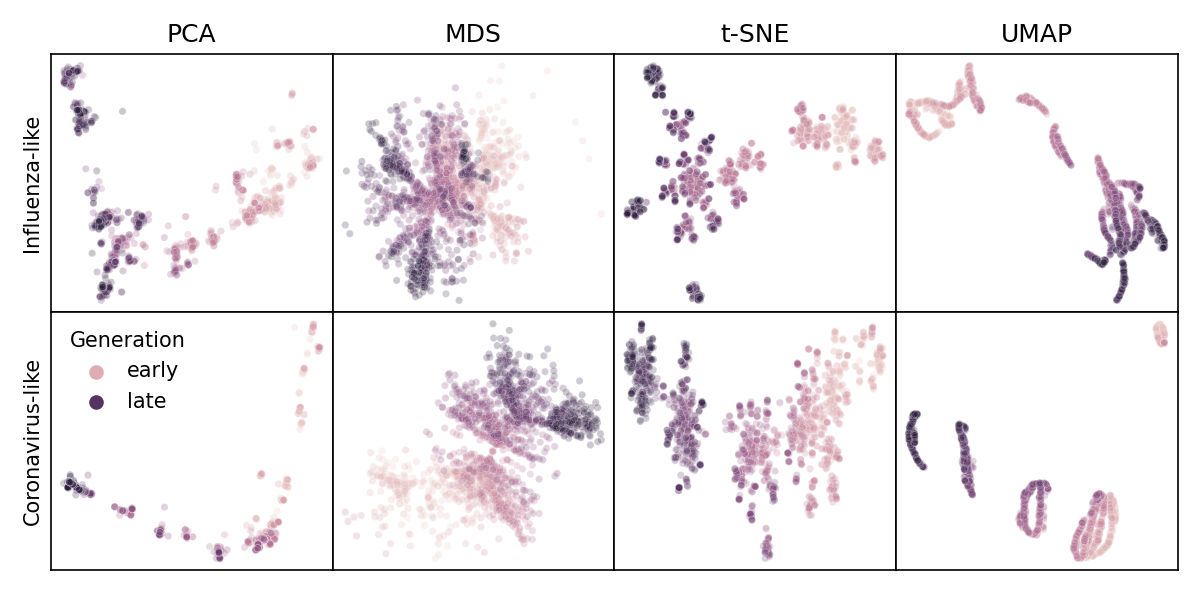
\includegraphics[width=\columnwidth]{figures/simulated-populations-representative-embeddings.png}
\caption{{\bf Representative embeddings for simulated populations using optimal parameters per pathogen (rows) and embedding method (columns).}
  Each panel represents an embedding method for a single replicate population for the corresponding pathogen type.
  Each point represents a simulated genome colored by its generation with darker values representing later generations.}
\label{fig:simulated-populations-representative-embeddings}
\end{figure}

% Place tables after the first paragraph in which they are cited.
\begin{table}[!ht]
%\begin{adjustwidth}{-2.25in}{0in} % Comment out/remove adjustwidth environment if table fits in text column.
\centering
\caption{
  {\bf Accuracy of embedding methods per human pathogenic virus sorted by normalized variation of information (VI) distance.}
  Threshold refers to the distance threshold used to assign clusters with HDBSCAN.}
\begin{tabular}{llrr}
\toprule
                     Pathogen & Method &   VI &  Threshold \\
\midrule
               Influenza H3N2 &  t-SNE & 0.04 &        2.0 \\
                              &   UMAP & 0.08 &        1.0 \\
                              &    MDS & 0.10 &        3.5 \\
                              &    PCA & 0.19 &        0.5 \\
SARS-CoV-2 (Nextstrain clade) &  t-SNE & 0.07 &        1.0 \\
                              &    MDS & 0.15 &        0.0 \\
                              &   UMAP & 0.16 &        0.5 \\
                              &    PCA & 0.22 &        0.5 \\
           SARS-CoV-2 (Pango) &  t-SNE & 0.12 &        1.0 \\
                              &    MDS & 0.23 &        0.0 \\
                              &   UMAP & 0.25 &        0.5 \\
                              &    PCA & 0.31 &        0.5 \\
\bottomrule
\end{tabular}

\label{table:accuracy}
%\end{adjustwidth}
\end{table}

\subsection*{Embedding clusters recapitulate phylogenetic clades for seasonal influenza A/H3N2}

Seasonal influenza A/H3N2's hemagglutinin (HA) sequences provide an ideal positive control to test dimensionality reduction methods and clustering.
A/H3N2's HA protein evolves rapidly, accumulating amino acid mutations that enable escape from adaptive immunity in human populations \cite{flu-review}.
These mutations produce distinct phylogenetic clades that represent potentially different antigenic phenotypes.
The World Health Organization (WHO) Global Influenza Surveillance and Response System (GISRS) regularly sequences genomes of circulating influenza lineages \cite{who-gisrs} and submits these sequences to public INSDC databases like NCBI's GenBank \cite{insdc}.
These factors, coupled with HA's relatively short gene size of 1,701 nucleotides, facilitate real-time genomic epidemiology of A/H3N2 \cite{nextflu,nextstrain} and rapid analysis by the embedding methods we wanted to evaluate.

We identified \jhc{NNN} A/H3N2 HA sequences from NCBI's GenBank database (methods) spanning from January 2016 to January 2020.
To evaluate the optimal parameters for each embedding method and avoid overfitting to specific datasets, we partitioned these data into a training dataset from 2016--2018 (N=\jhc{NNN} sequences) and a test dataset from 2018--2020 (N=\jhc{NNN} sequences).
We first analyzed the training data with Nextstrain's seasonal influenza workflow that creates a multiple sequence alignment, infers a time-resolved phylogenetic tree, and assigns clade labels to each sequence based on our own expert-defined clade annotations \cite{nextstrain,seasonal-flu,augur}.
We applied each embedding method to the multiple sequence alignment, identified clusters in the embeddings with HDBSCAN \cite{hdbscan}, and evaluated the accuracy of cluster classifications compared to known clade annotations.
We applied this general approach in an exhaustive grid search to identify the optimal parameters for each combination of embedding method and HDBSCAN (see Methods).

All four embedding methods qualitatively recapitulated clade-level groupings observed in the phylogeny (Fig~\ref{fig:seasonal-influenza-h3n2-ha-embeddings}).
Strains from the same clade generally grouped tightly together in PCA, t-SNE, and UMAP embeddings.
While MDS followed this general pattern, it also produced separate pairs of A3 and A4 clusters that did not correspond to meaningful subclades.
All of the embedding methods clearly delineated larger phylogenetic clades into separate spaces (e.g., A1 and A2) and, with the exception of t-SNE, placed related subclades closer together (e.g., A2 and A2/re or the A1b subclades).
The t-SNE embedding placed distantly related pairs of clades like 3c3.A and A2 as close together as closely-related clades like A2 and its subclade A2/re.
These results suggest that t-SNE maintains both local and global structure, but that our interpretation of the absolute distance between points in these embeddings cannot be linear.

% For figure citations, please use "Fig" instead of "Figure".

% Place figure captions after the first paragraph in which they are cited.
\begin{figure}[!h]
% TODO: remove includegraphics commands in final submission; figures must be uploaded separately from the manuscript.
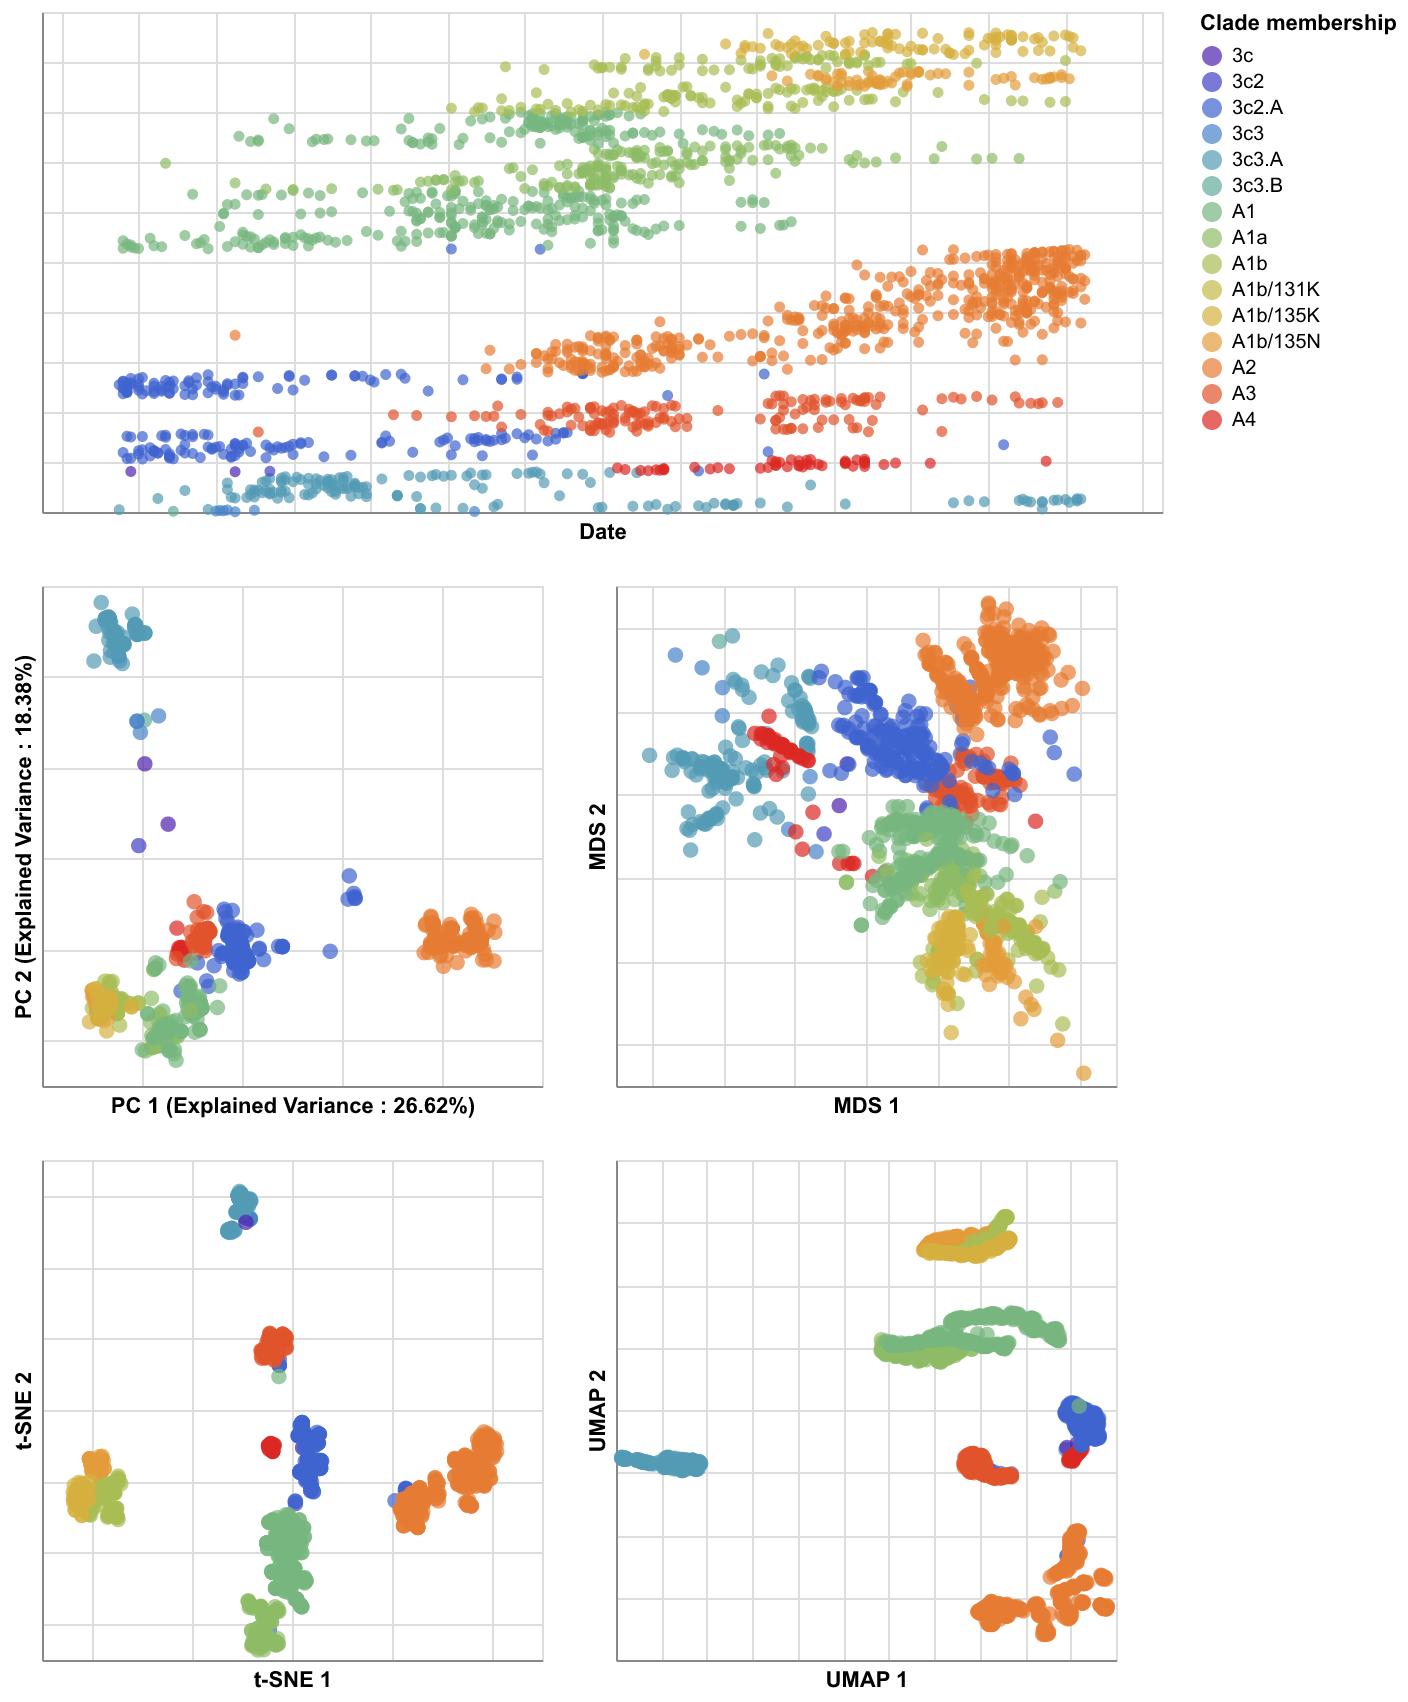
\includegraphics[width=\columnwidth]{figures/flu-2016-2018-ha-embeddings-by-clade.png}
\caption{{\bf The phylogeny of influenza A/H3N2 viruses (top) shows the evolutionary relationships among viruses including clades, or viruses that share the same mutations and descend from the same common ancestor.}
Reduced dimensionality embeddings of genetic sequences into two dimensions by PCA (middle left), MDS (middle right), t-SNE (bottom left), and UMAP (bottom right) generally recapitulate groups of viruses into clades without inferring ancestral relationships.}
\label{fig:seasonal-influenza-h3n2-ha-embeddings}
\end{figure}

To quantify the apparent maintenance of local and global structure in these embeddings, we calculated the relationship between pairwise genetic distance of genomes and pairwise Euclidean distance of those genomes in each embedding.
All four methods maintained a linear relationship between genetic and Euclidean distances for genomes that differed by no more than $\approx$20 nucleotides (Fig~\ref{fig:seasonal-influenza-h3n2-ha-pairwise-distances}).
However, PCA and MDS were the only methods that consistently maintained that linearity as genetic distance increased (Pearson's $R^{2} = 0.767 \pm 0.000$  and $0.849 \pm 0.000$, respectively).
In contrast, the relationship between genetic and Euclidean distance was nonlinear in t-SNE (Pearson's $R^{2} = 0.393 \pm 0.001$) and UMAP (Pearson's $R^{2} = 0.397 \pm 0.000$) embeddings.
Genomes that differed by more than $\approx$20 nucleotides were equally as likely to map close together as far apart in these embeddings.

\begin{figure}[!h]
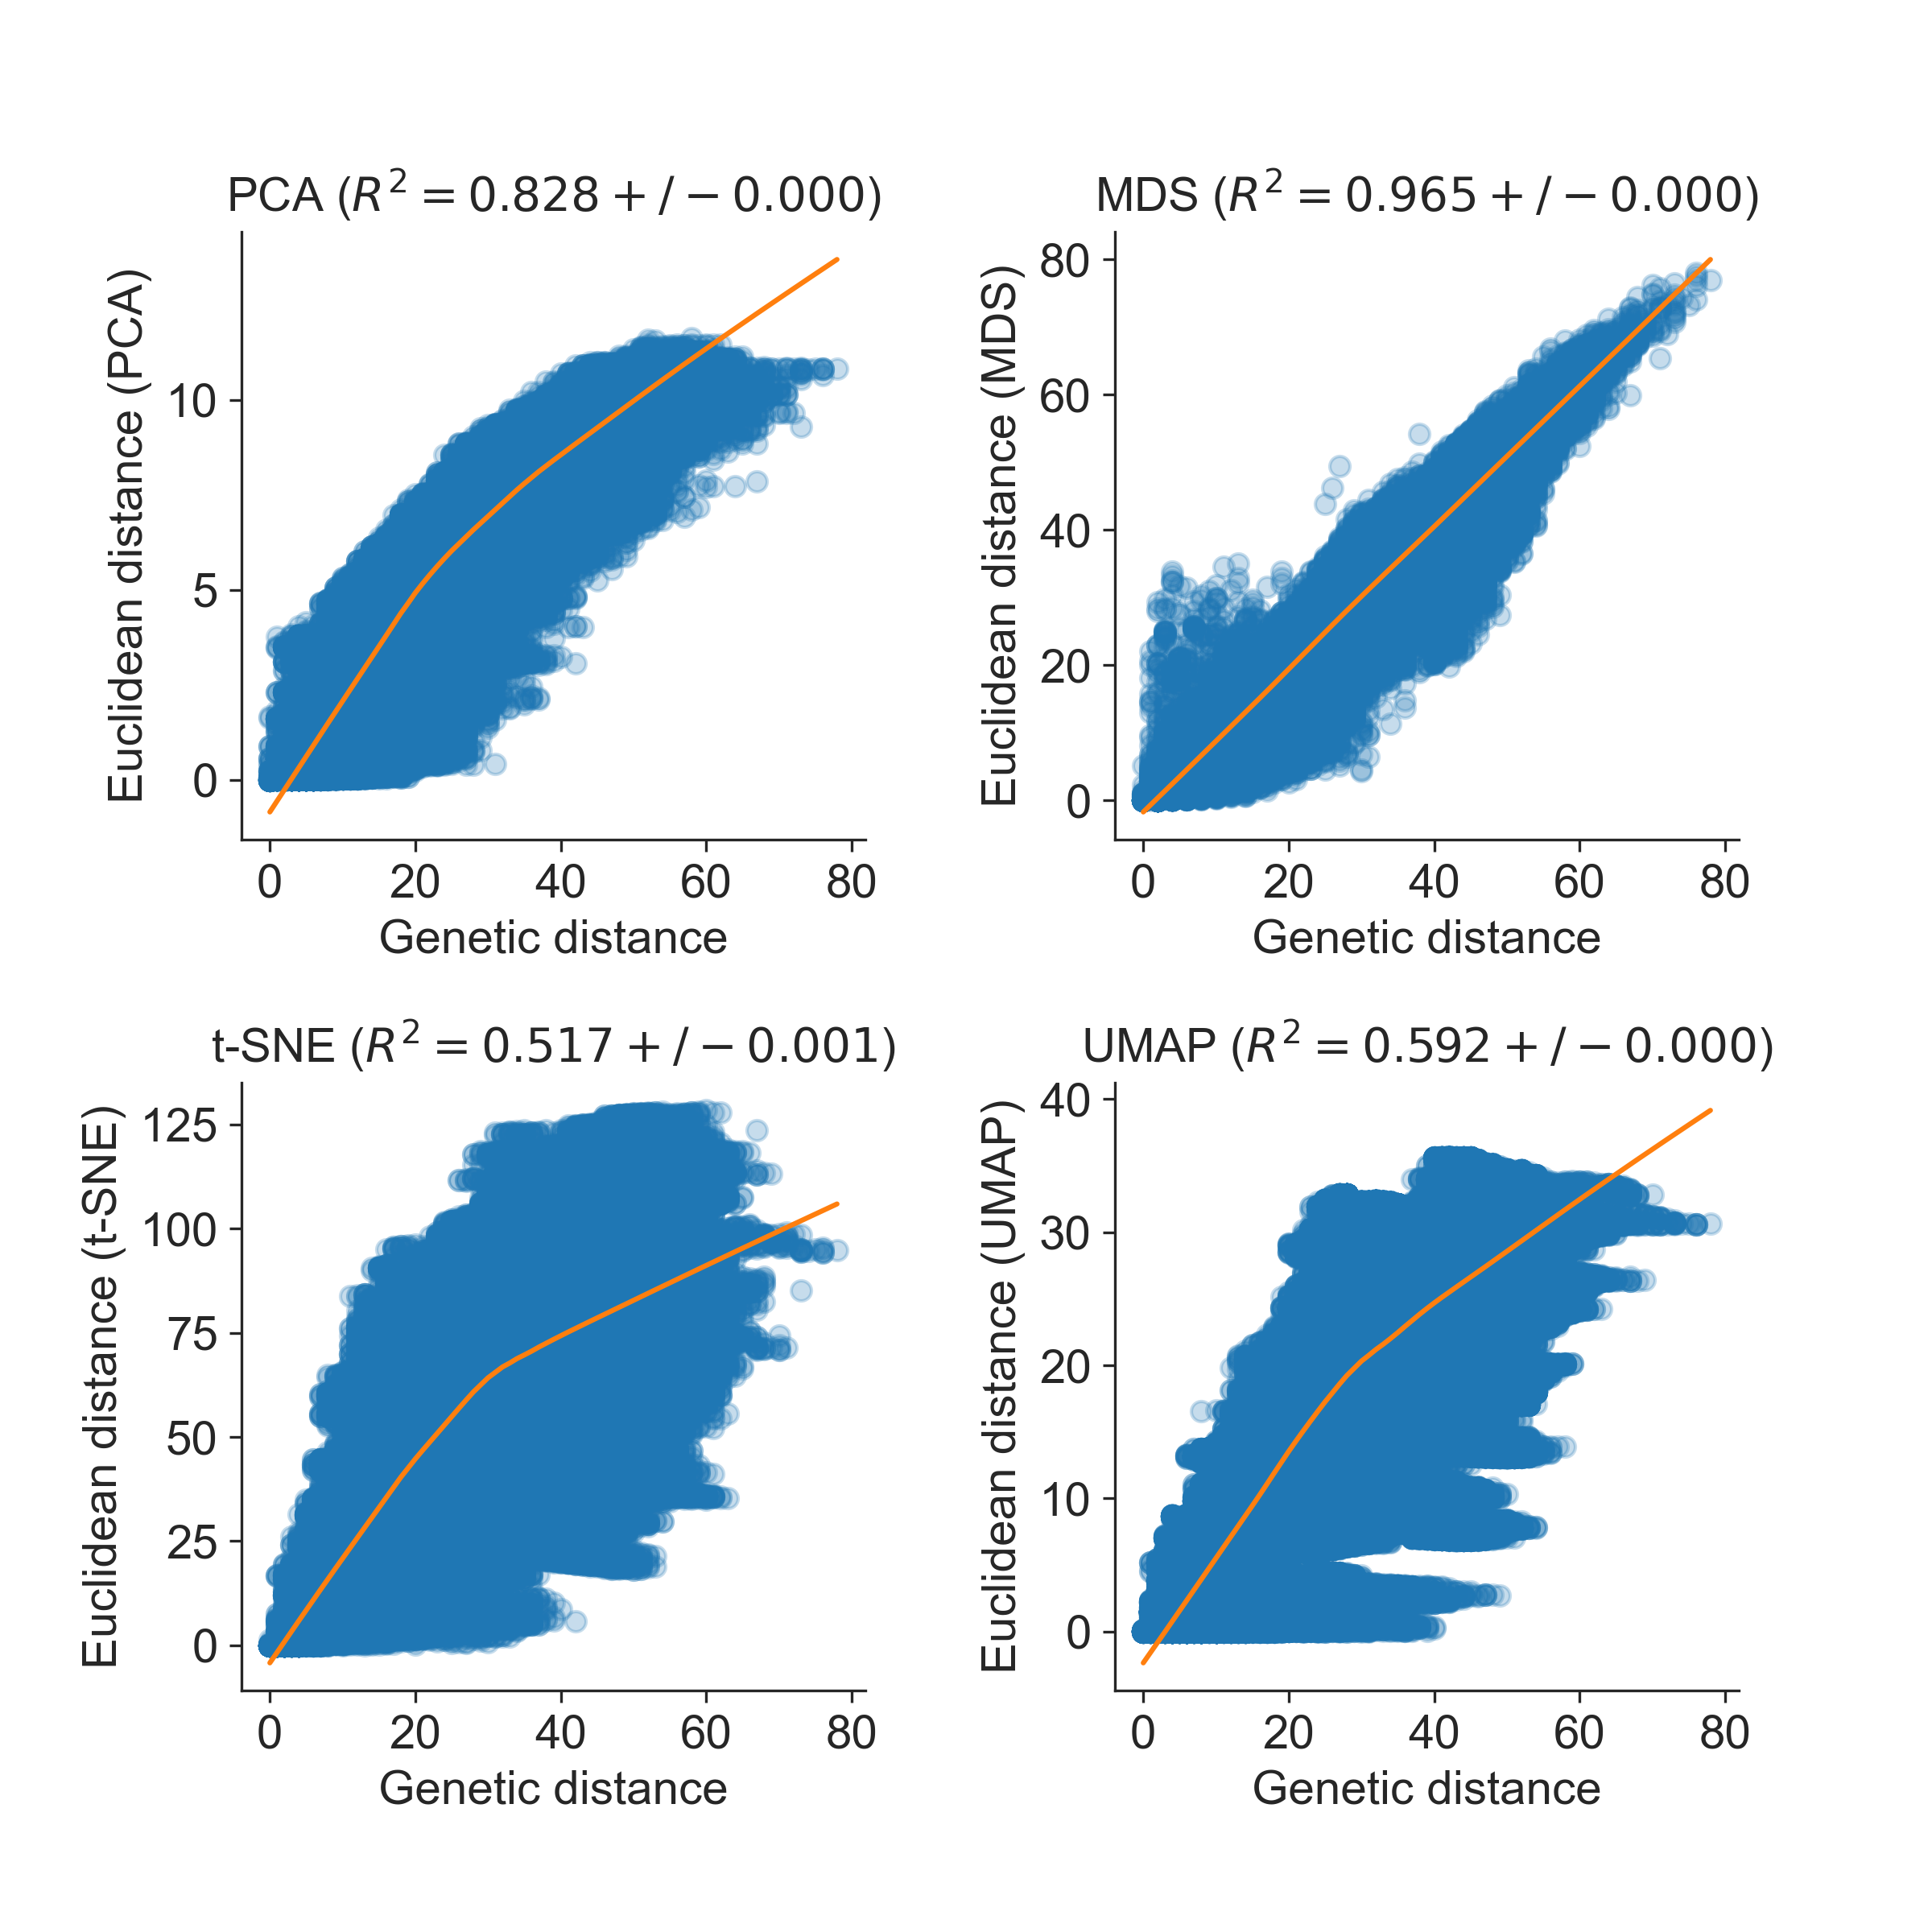
\includegraphics[width=\columnwidth]{figures/flu-2016-2018-ha-euclidean-distance-by-genetic-distance.png}
\caption{{\bf The mapping between Euclidean and Genetic distance assess the strength of both the local and global structure of the embedding recapitulation.}
The scatterplot for PCA (upper left), MDS (upper right), t-SNE (lower left), and UMAP (lower right) consistently exhibit linear relationships for pairs of strains that differ by around 20 nucleotides.}
\label{fig:seasonal-influenza-h3n2-ha-pairwise-distances}
\end{figure}

Next, we measured how well clusters of genomes in a given embedding corresponded to our expert clade annotations.
For each embedding described above, we applied hierarchical clustering with HDBSCAN to assign cluster labels to each genome.
For each pair of genomes, we tested whether both genomes belonged to the same clade and the same cluster.
We calculated the accuracy of cluster labels using the Matthew's correlation coefficient (MCC) of the resulting pairwise tests \cite{matthews_1975}.
Since we previously identified the optimal HDBSCAN parameter based on this same accuracy metric and dataset, we anticipated that the cluster accuracy would be relatively high.
We counted genomes that HDBSCAN could not assign to a cluster as false negatives in our MCC calculation, but we also used this number of unassigned genomes as an additional metric of cluster quality.

As expected, the clusters for each method generally corresponded to larger phylogenetic clades (Fig~\ref{fig:seasonal-influenza-h3n2-ha-clusters}, Table~\ref{table:accuracy}).
The t-SNE embedding produced the most accurate classification (MCC = 0.756) with 20 clusters and \jhc{NNN} genomes not assigned to a cluster.
UMAP also accurately classified genomes (MCC = 0.662) with only five clusters and no unassigned genomes.
PCA (MCC = 0.368) and MDS (MCC = 0.476) both performed relatively poorly but for different reasons.
PCA combined genomes from divergent phylogenetic clades A1 and A2 into the same larger cluster (cluster 4) but managed to assign clusters to all but \jhc{NNN} genomes.
In contrast, MDS distinguished between most large clades including 3c3.A, A1, and A2, but it also placed closely-related strains from the same clades in two separate clusters (clusters 0 and 5) and failed to assign clusters to \jhc{NNN} genomes.
Clusters 0 and 5 correspond to the apparently arbitrary splitting of both clades A3 and A4 into different groups in MDS space described above.
These results indicate that nonlinear embeddings of t-SNE and UMAP could be better-suited for clustering and classification than linear embeddings from PCA and MDS.

\begin{figure}[!h]
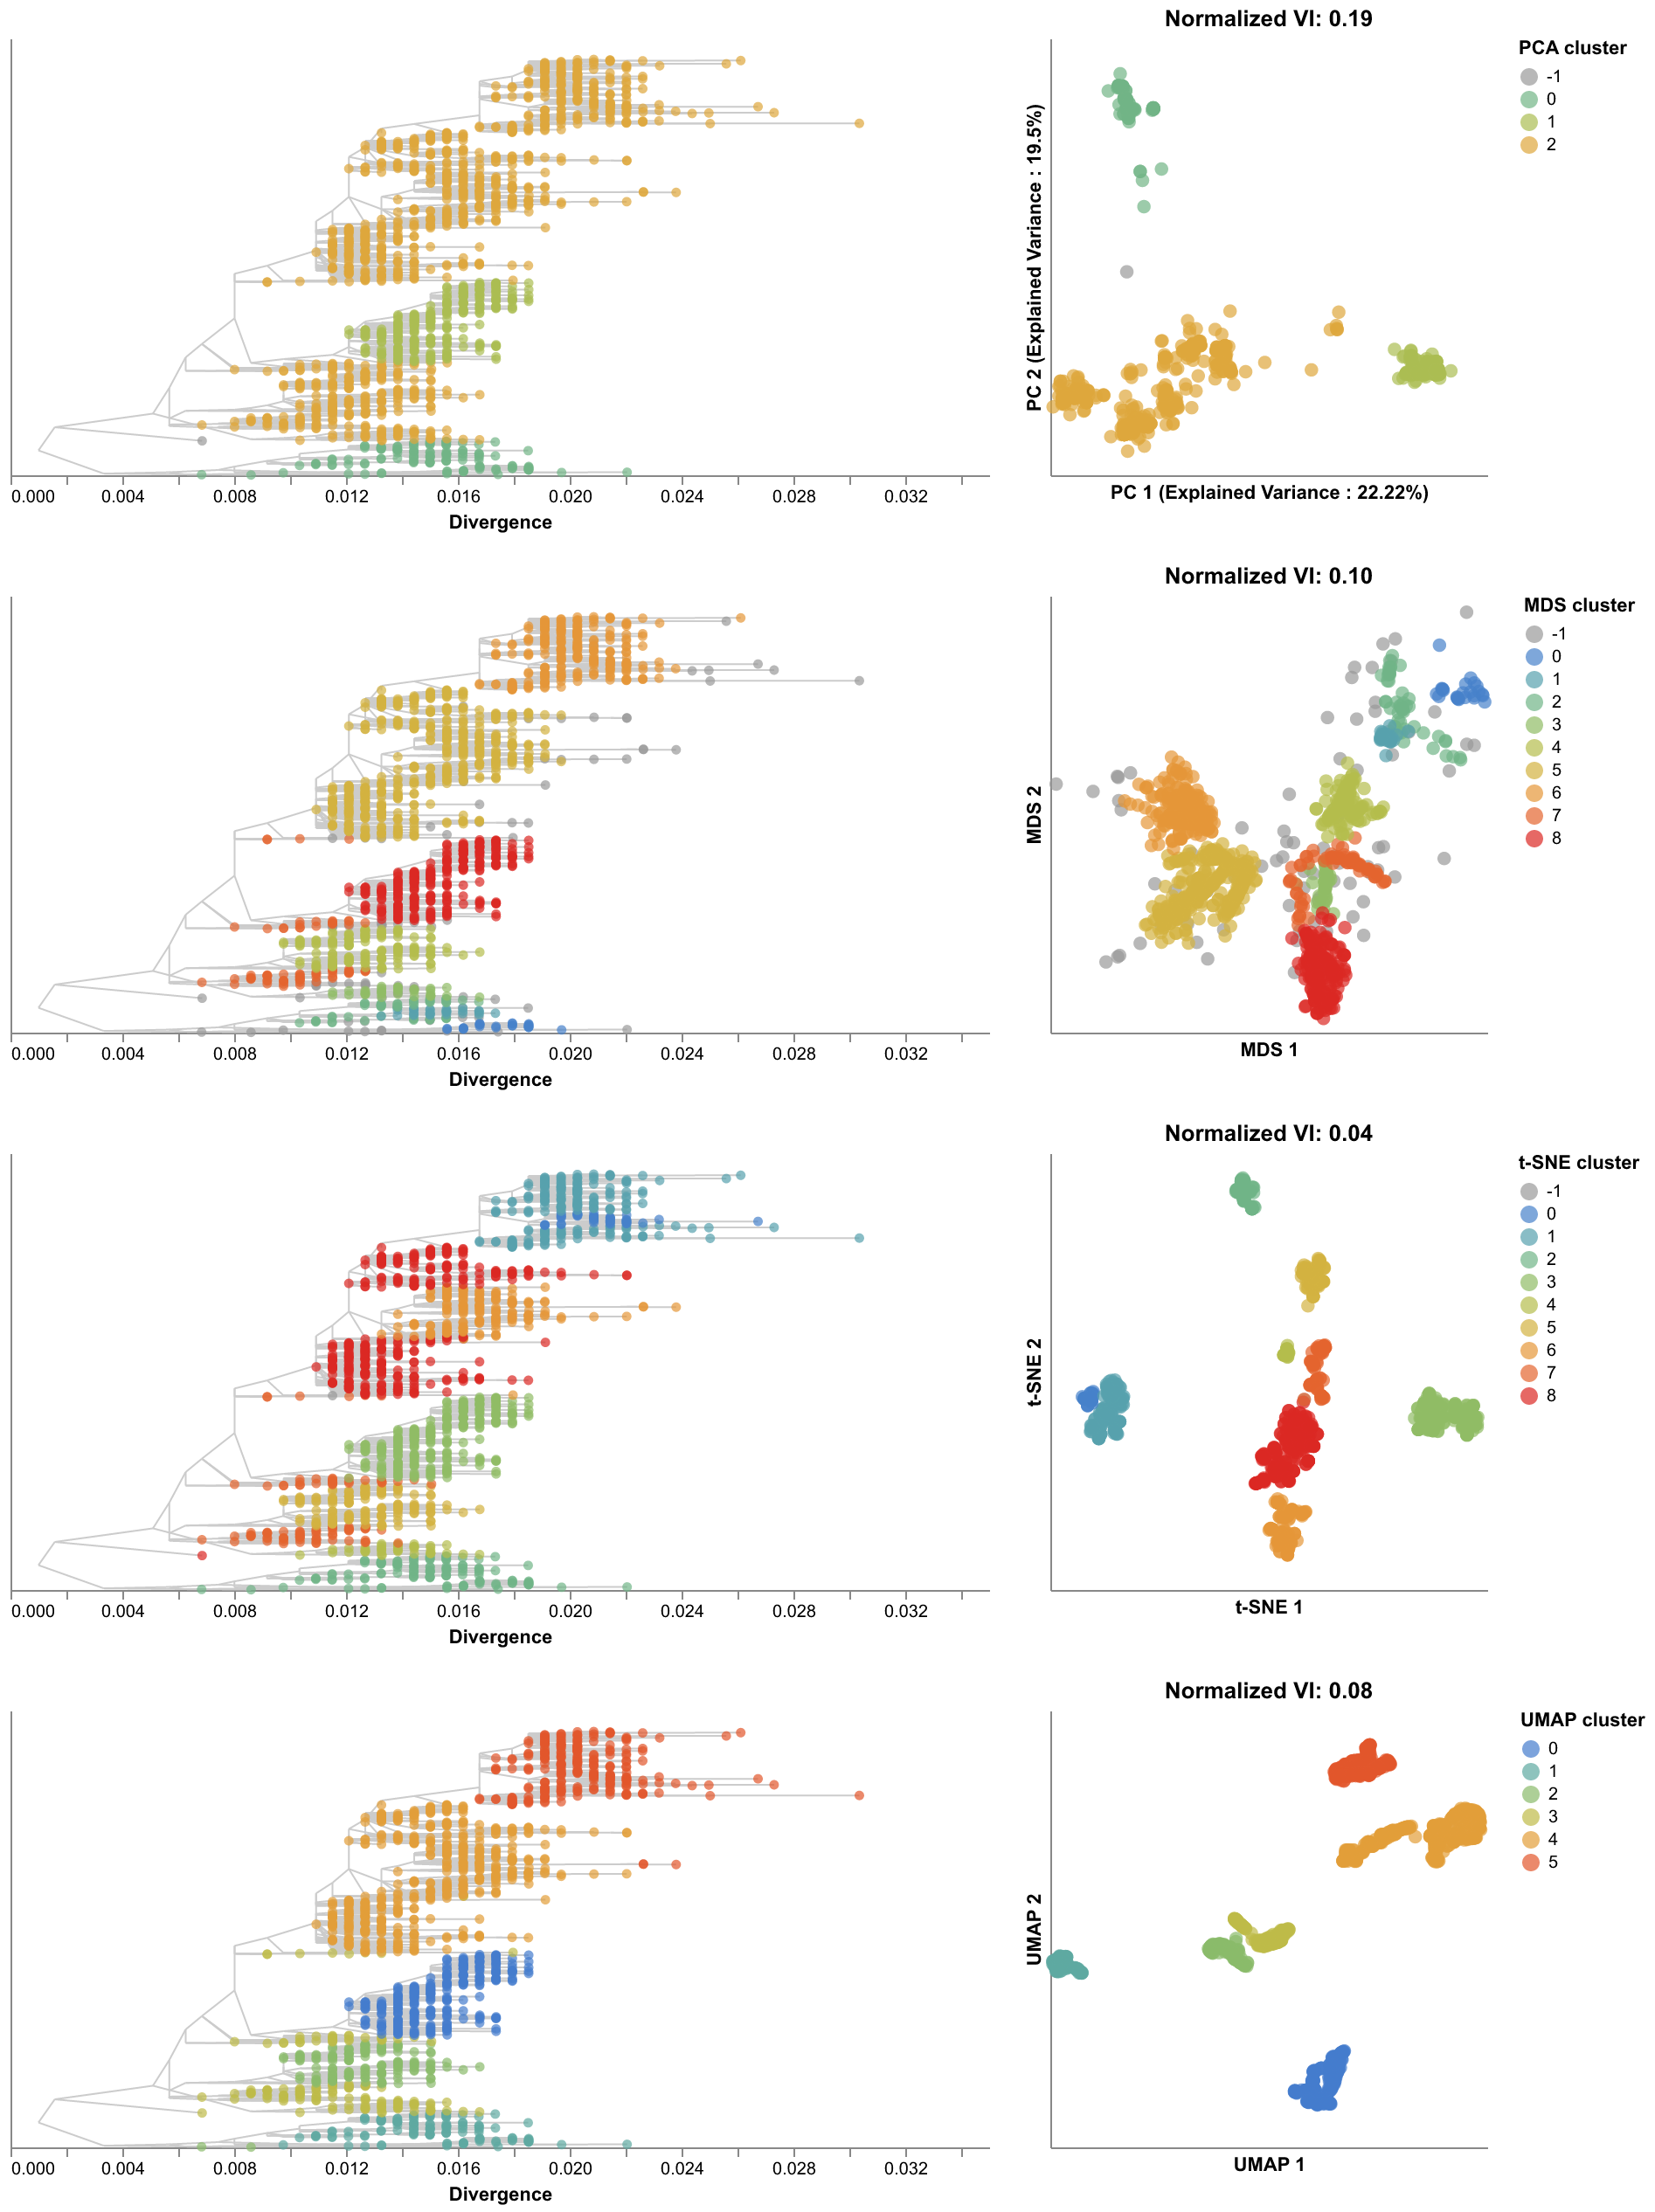
\includegraphics[width=\columnwidth]{figures/flu-2016-2018-ha-embeddings-by-cluster.png}
\caption{{\bf The embeddings colored by their HDBSCAN label, with the distance threshold defined by the threshold that preserved the greatest amount of clade relationships.}
The chart for PCA (top left), MDS (middle left), t-SNE (middle left), and UMAP (bottom left) generally recapitulate groups of viruses into clades without inferring ancestral relationships, and the trees on the righthand side describes how these clade grouping appear on the tree, which does infer ancestral relations.}
\label{fig:seasonal-influenza-h3n2-ha-2016-2018-clusters}
\end{figure}

To understand whether these embedding methods could be used to cluster previously unseen genomes for the same virus, we applied each method to the test dataset spanning 2018--2020, clustered genomes in the embedding space with HDBSCAN, and calculated the accuracy of the cluster assignments based on previously defined clades.

\begin{figure}[!h]
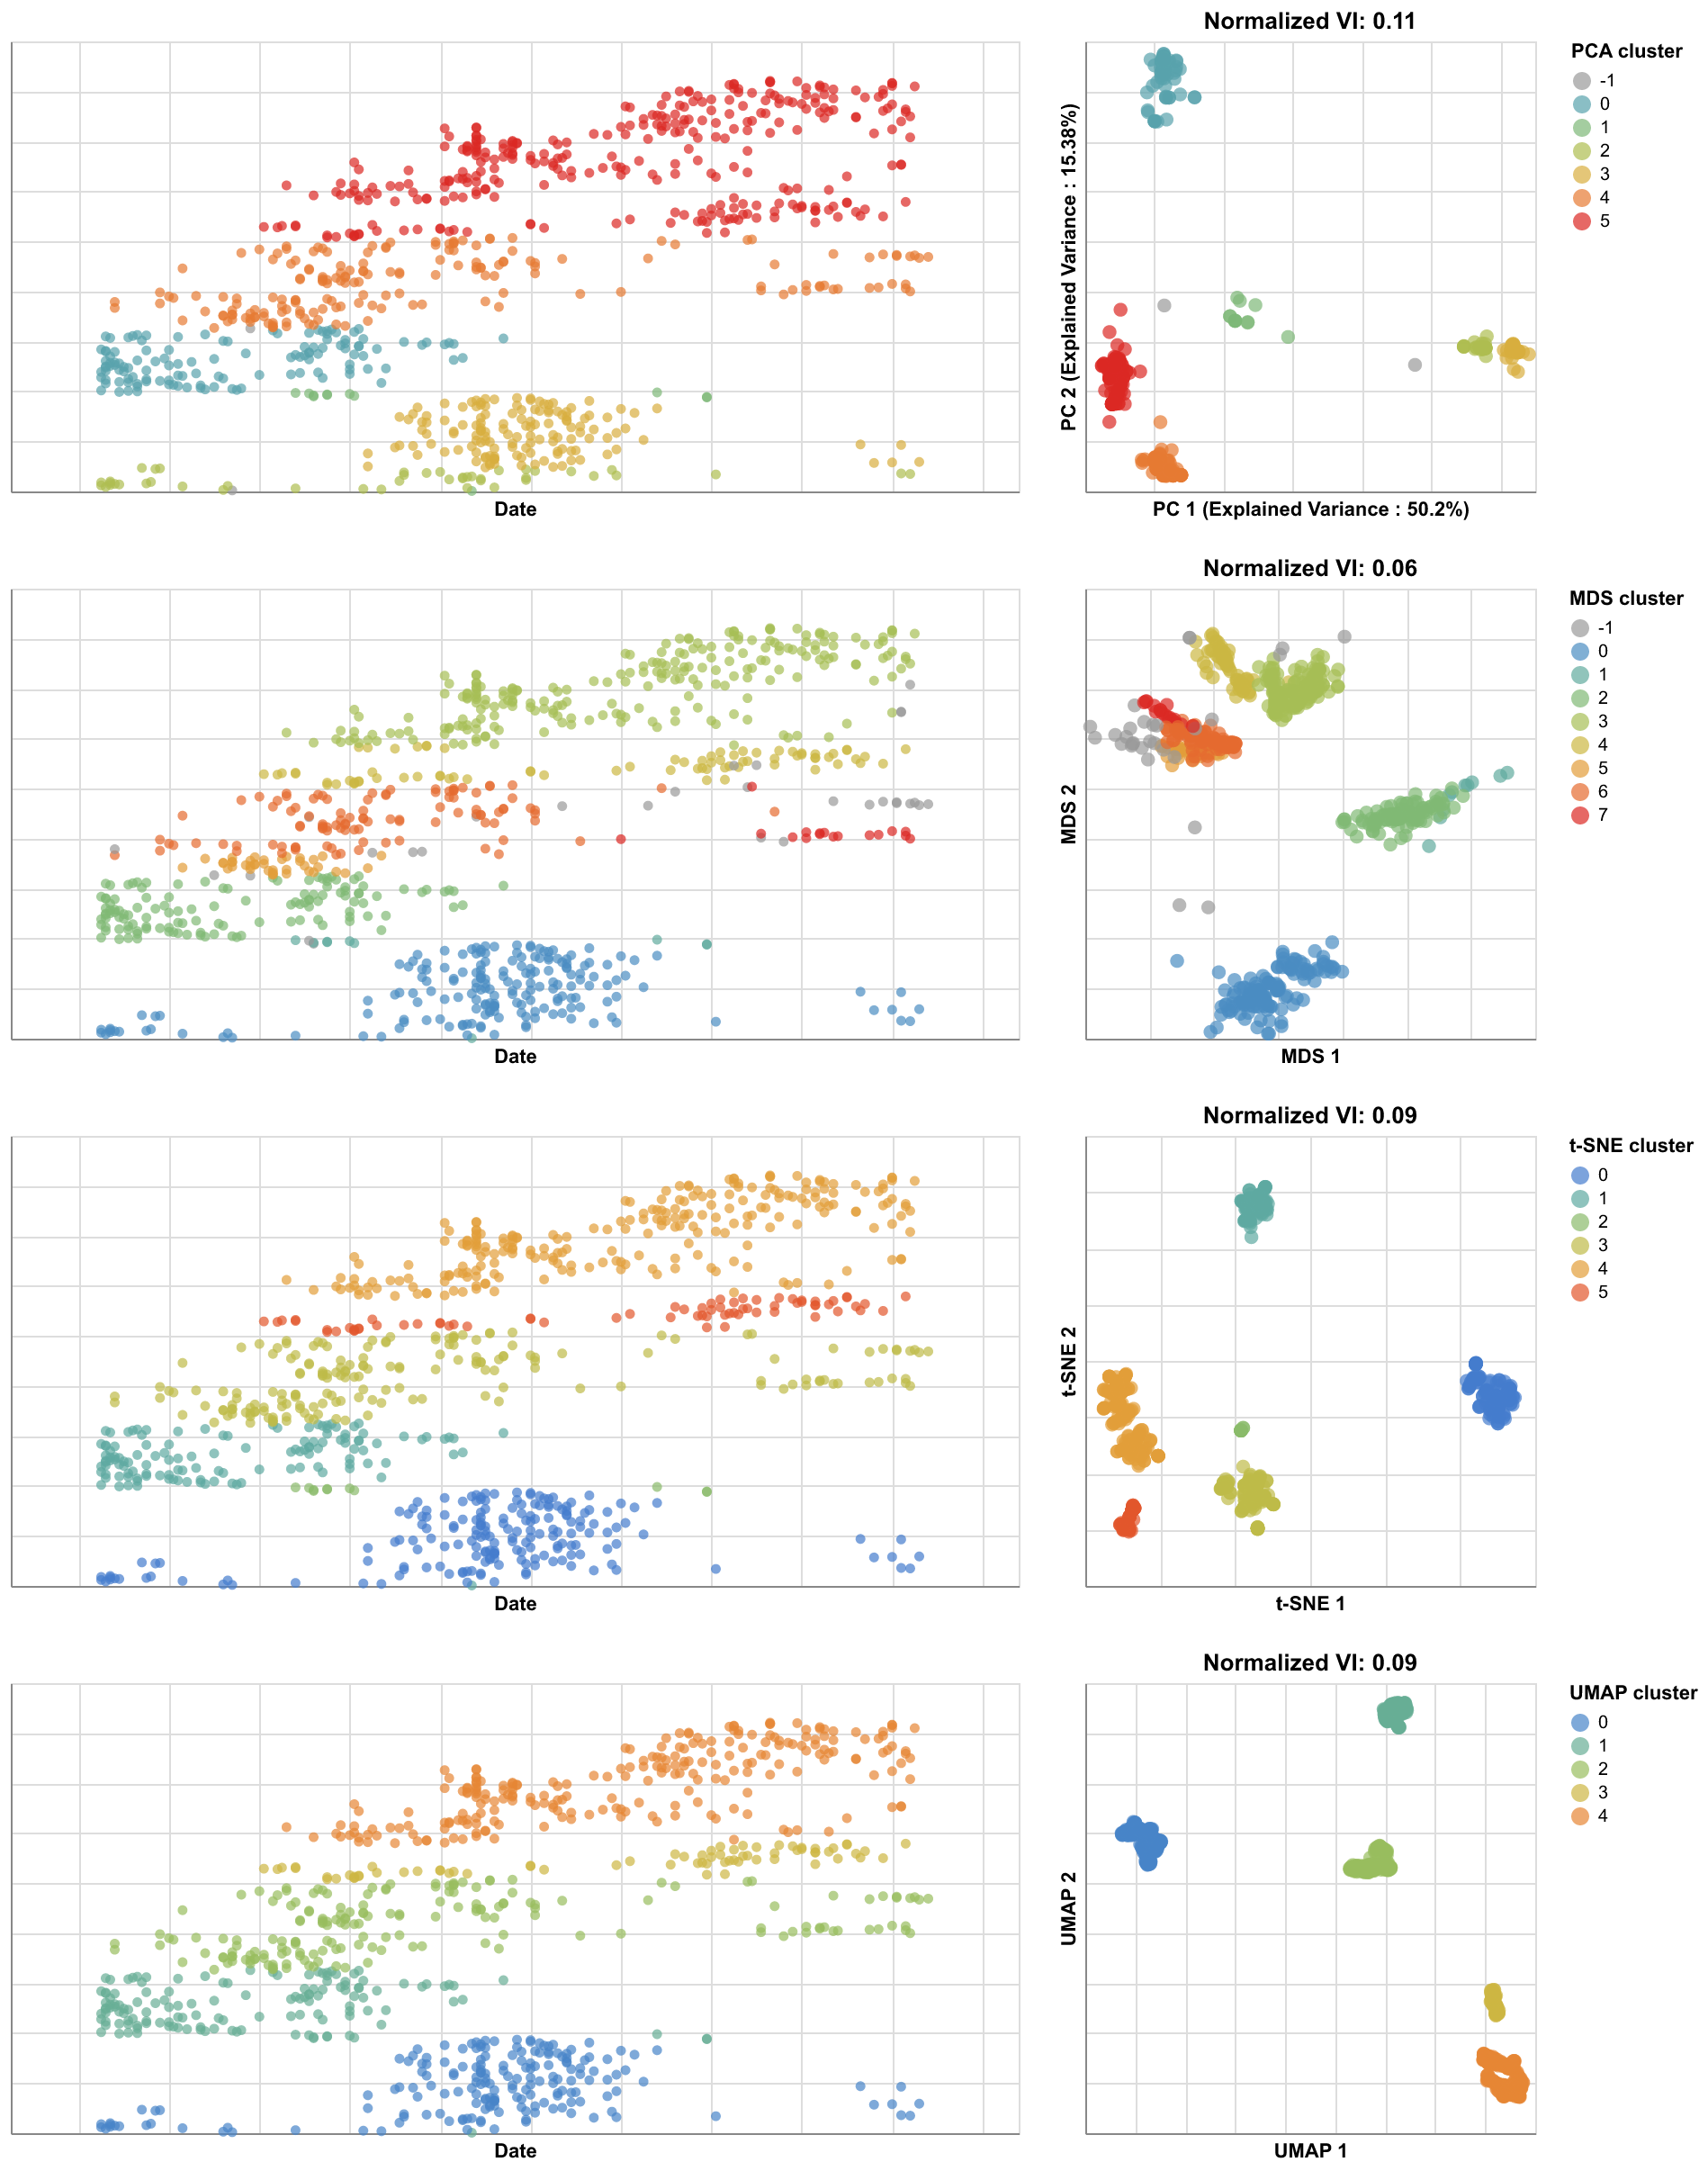
\includegraphics[width=\columnwidth]{figures/flu-2018-2020-ha-embeddings-by-cluster.png}
\caption{{\bf The embeddings colored by their HDBSCAN label, with the distance threshold defined by the threshold that preserved the greatest amount of clade relationships.}
The chart for PCA (top left), MDS (middle left), t-SNE (middle left), and UMAP (bottom left) generally recapitulate groups of viruses into clades without inferring ancestral relationships, and the trees on the righthand side describes how these clade grouping appear on the tree, which does infer ancestral relations.}
\label{fig:seasonal-influenza-h3n2-ha-2018-2020-clusters}
\end{figure}

\subsection*{Joint embeddings of hemagglutinin and neuraminidase genomes identify seasonal influenza virus A/H3N2 reassortment events}

\begin{figure}[!h]
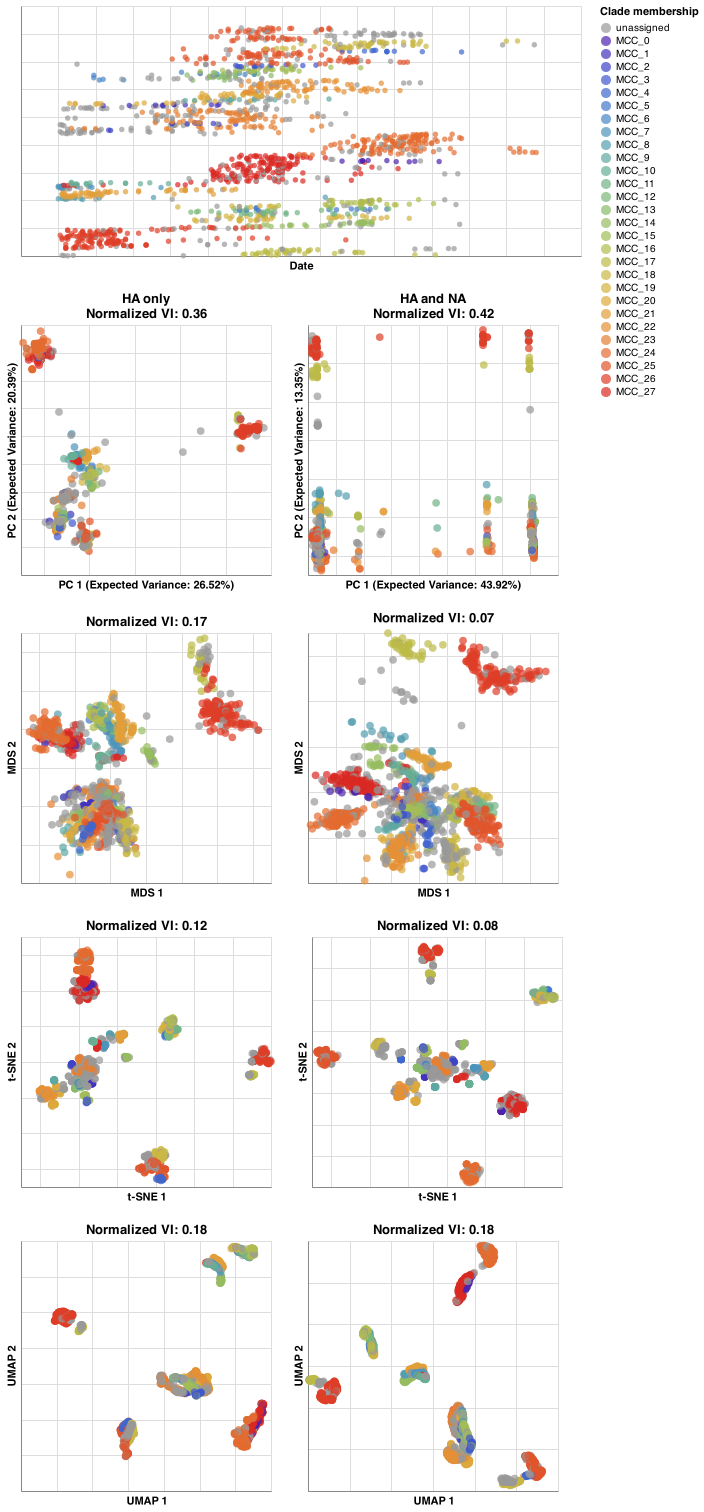
\includegraphics[width=\columnwidth]{figures/flu-2016-2018-ha-na-embeddings-by-mcc.png}
\caption{{\bf Embeddings of seasonal influenza HA-only (first column) and concatenated HA/NA sequences (second column) colored by TreeKnit Maximally Compatible Clades (MCC) label.}
}
\label{fig:seasonal-influenza-h3n2-ha-na-2016-2018-embeddings}
\end{figure}

\subsection*{SARS-CoV-2 clusters recapitulate emerging lineage designations}

\begin{figure}[!h]
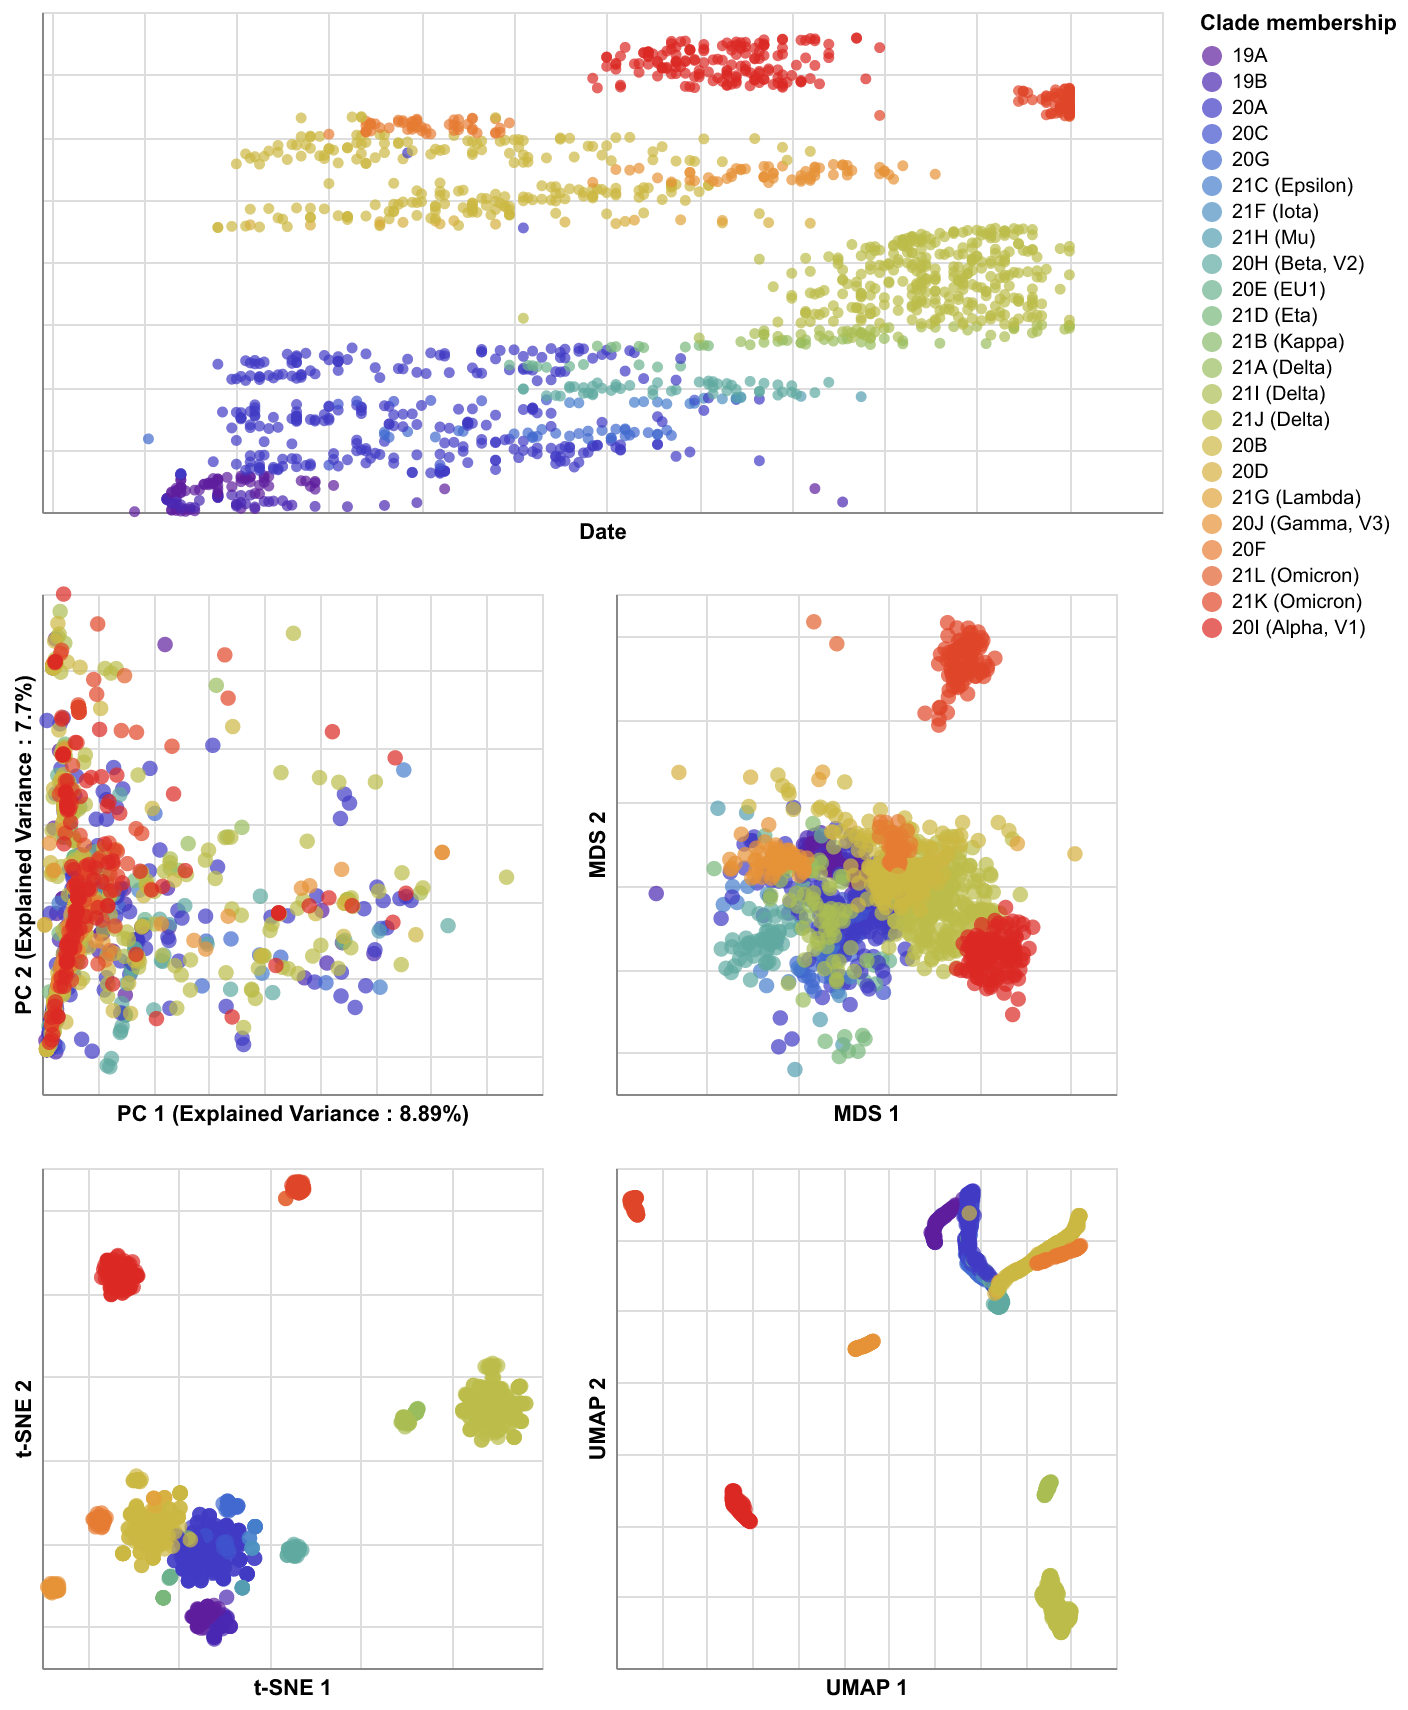
\includegraphics[width=\columnwidth]{figures/sarscov2-embeddings-by-Nextstrain_clade-clade.png}
\caption{{\bf Embeddings of SARS-CoV-2 sequences collected between January 1, 2020 and January 1, 2021 colored by Nextstrain clade label.}
}
\label{fig:sars-cov-2-2020-2021-embeddings}
\end{figure}

\begin{figure}[!h]
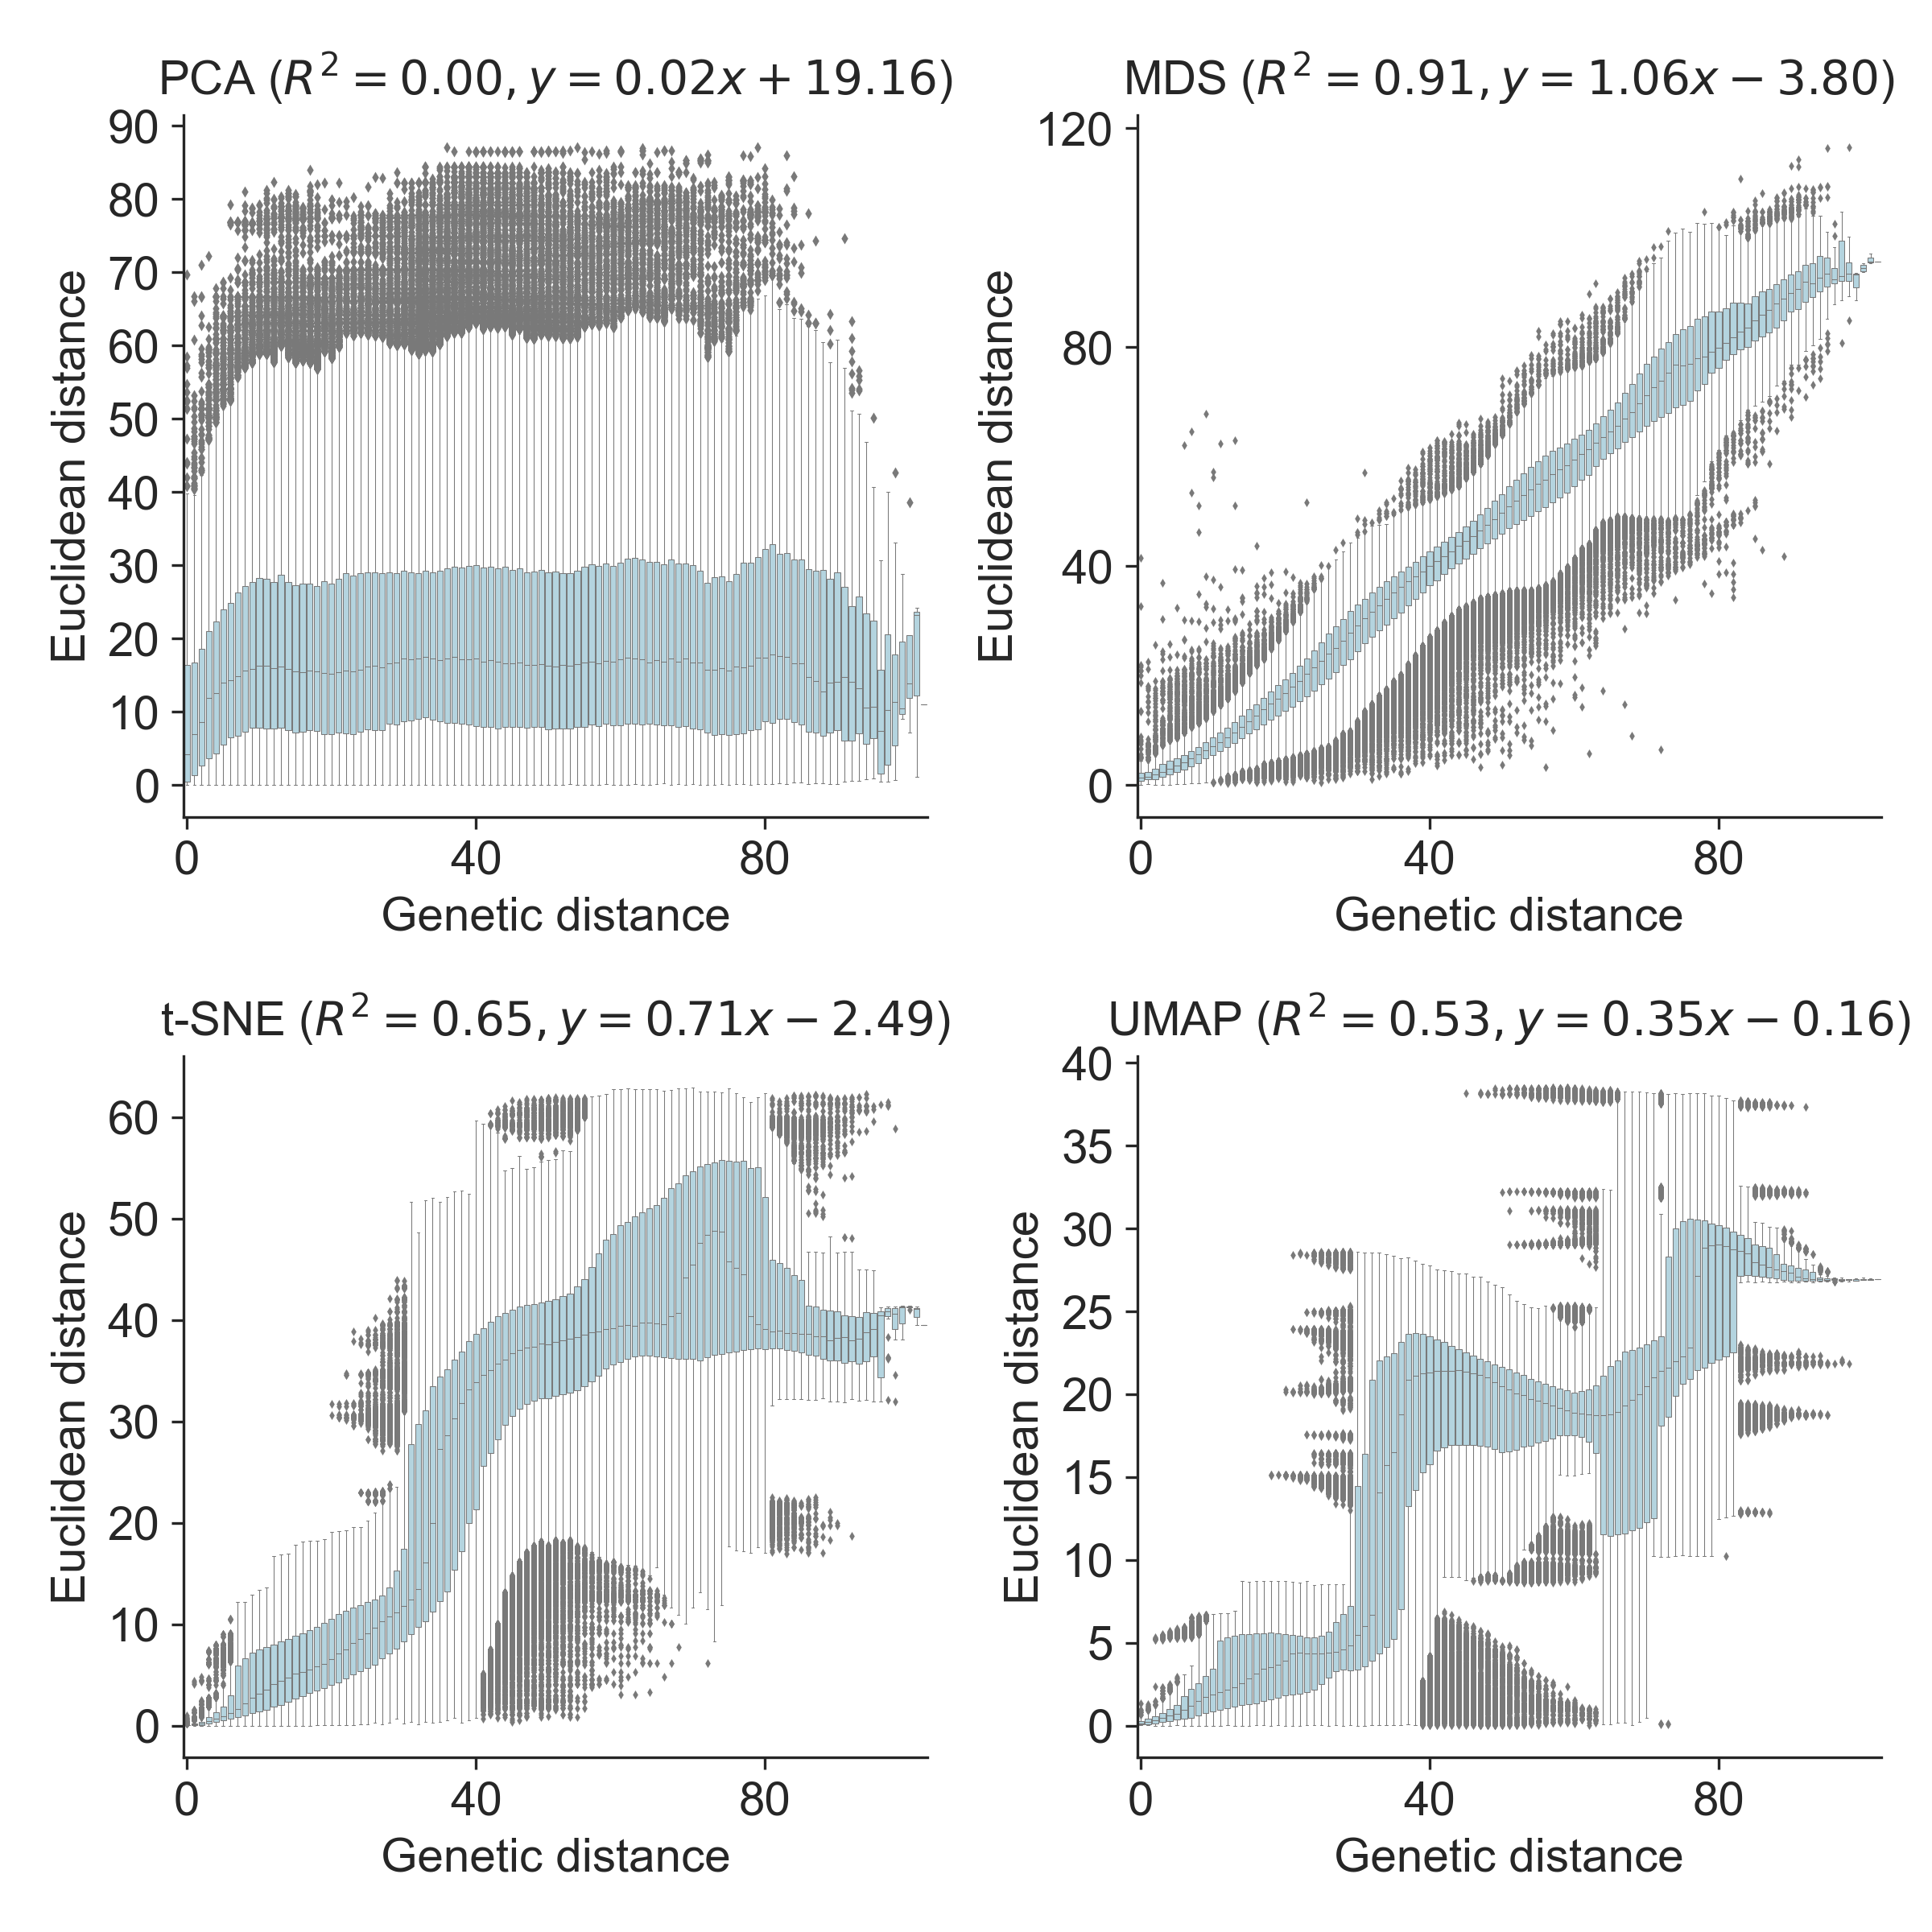
\includegraphics[width=\columnwidth]{figures/sarscov2-euclidean-distance-by-genetic-distance.png}
\caption{{\bf The mapping between Euclidean and genetic distance assess the strength of both the local and global structure of the embedding recapitulation.}
The scatterplot for PCA (upper left), MDS (upper right), t-SNE (lower left), and UMAP (lower right) consistently exhibit linear relationships for pairs of strains that differ by around 20 nucleotides.}
\label{fig:sars-cov-2-pairwise-distances}
\end{figure}

\begin{figure}[!h]
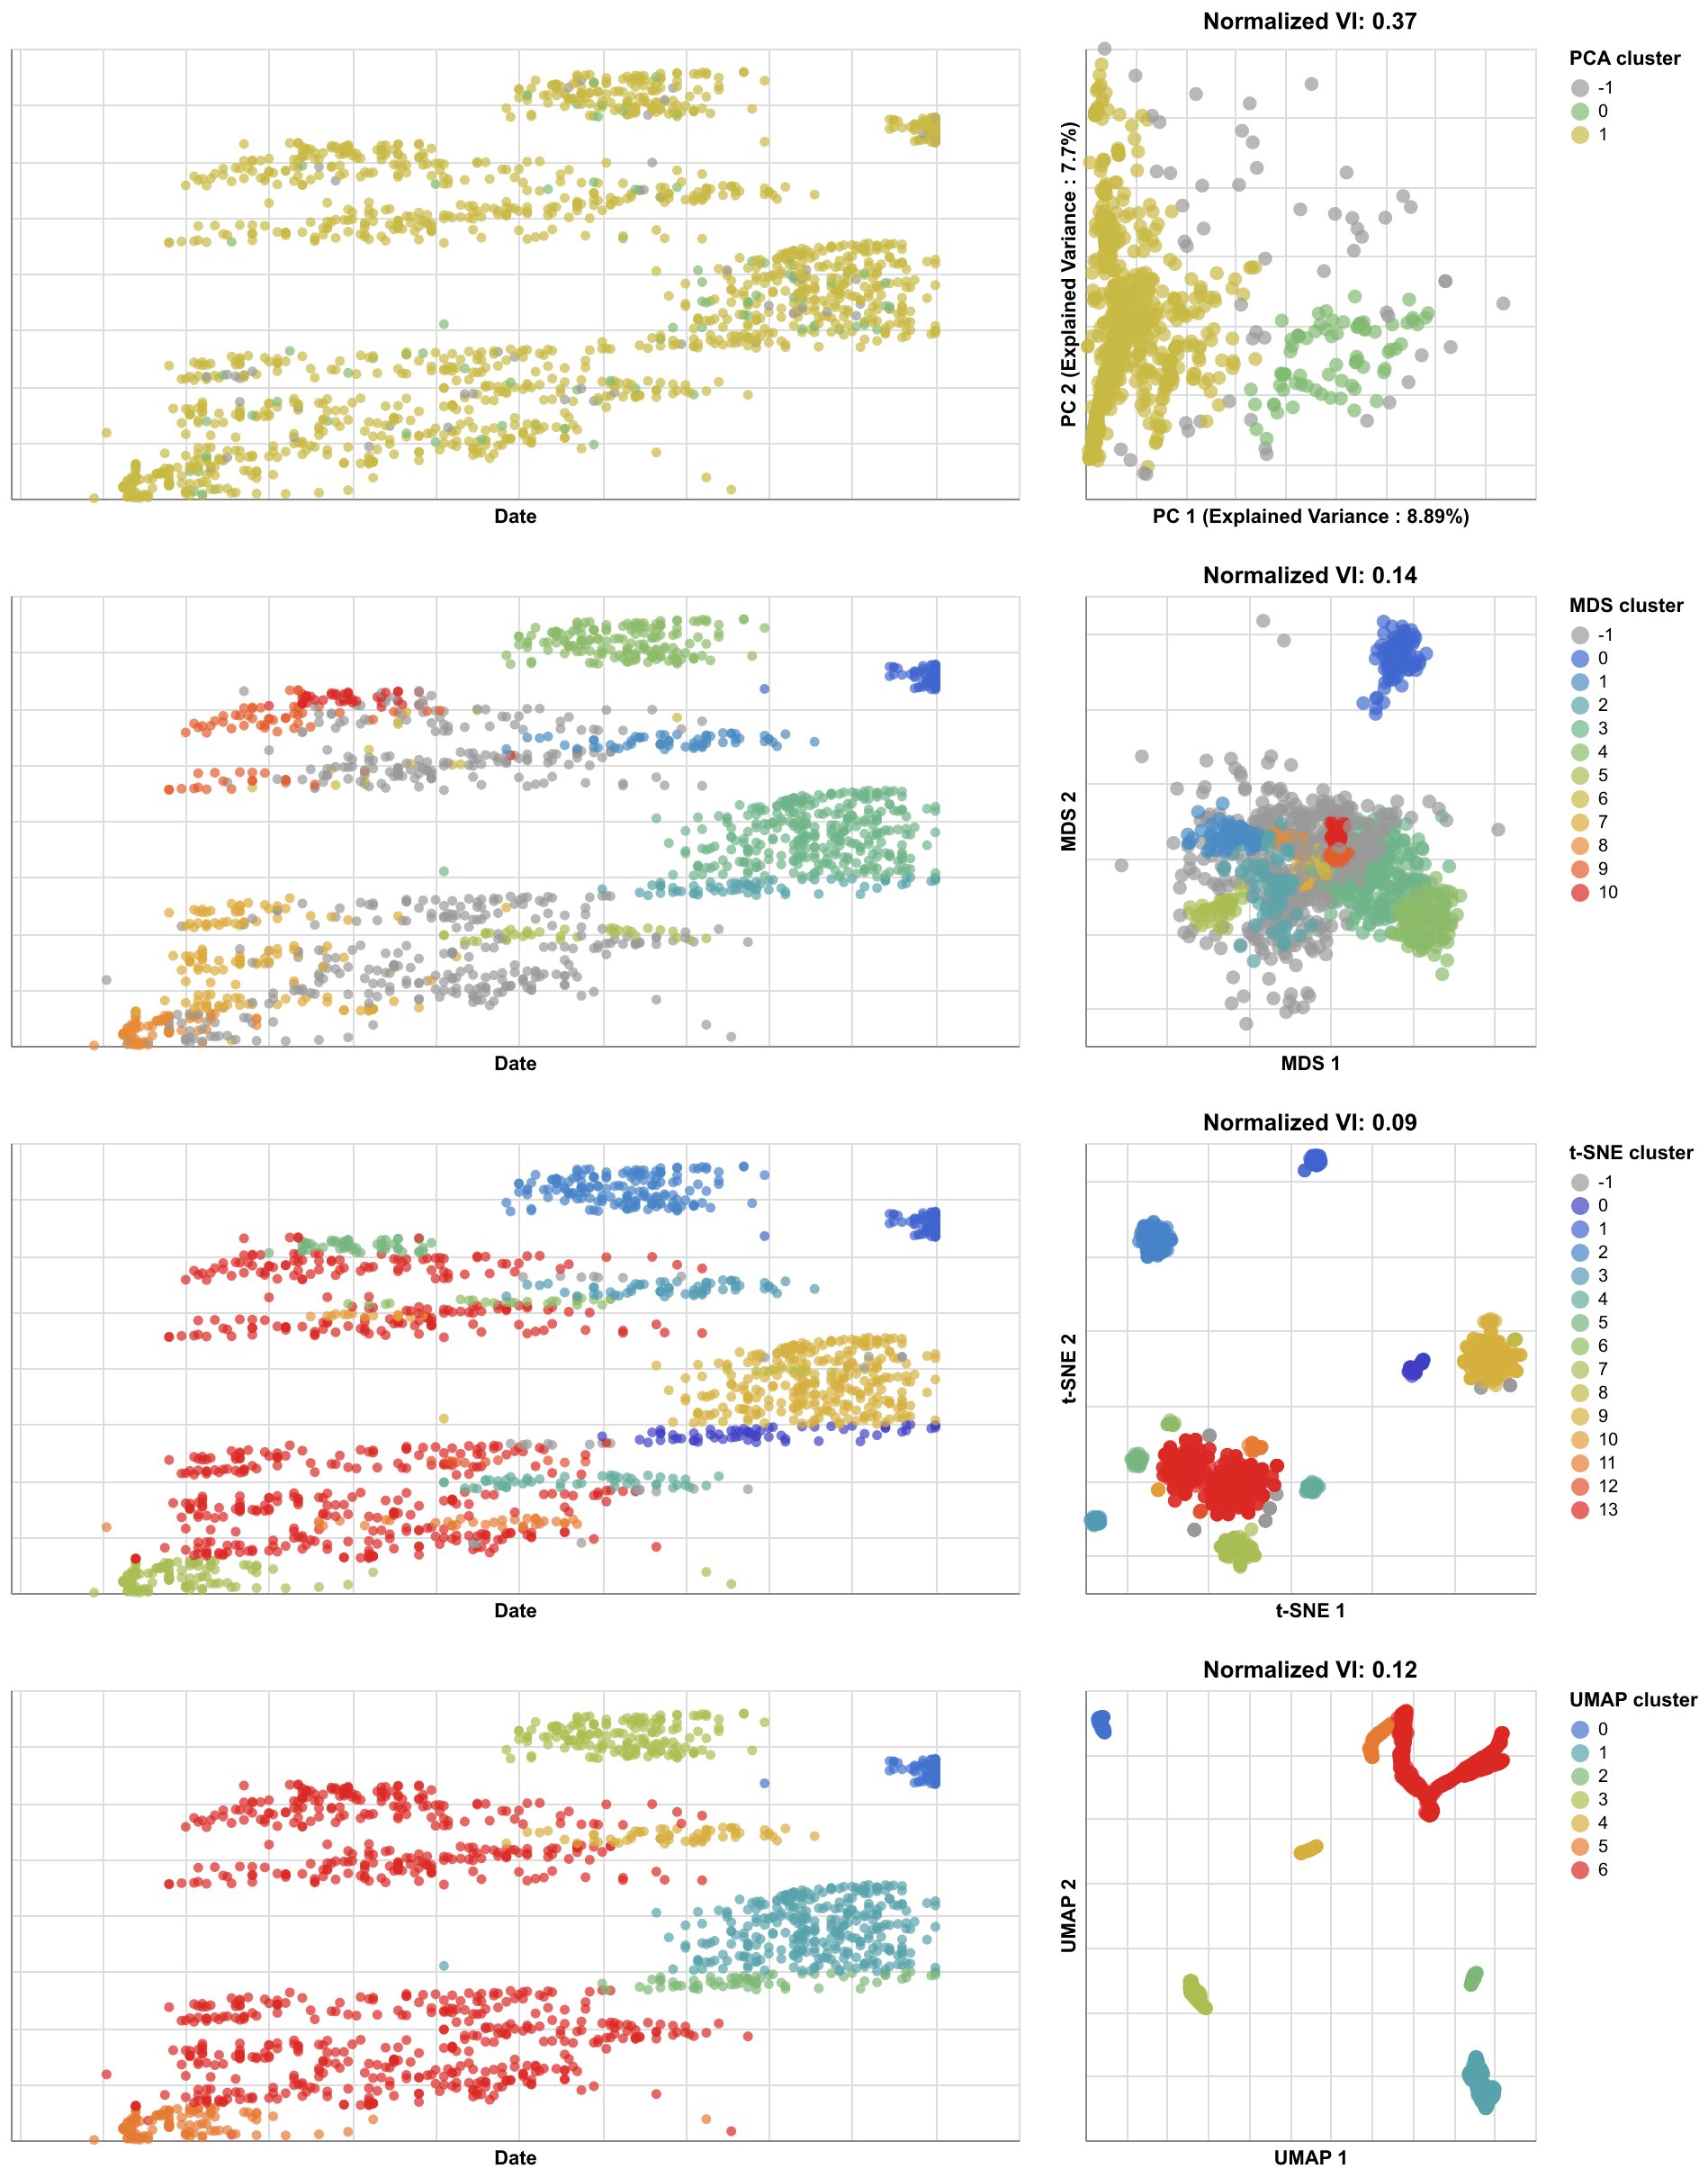
\includegraphics[width=\columnwidth]{figures/sarscov2-embeddings-by-cluster-vs-Nextstrain_clade.png}
\caption{{\bf Embeddings of SARS-CoV-2 sequences collected between January 1, 2020 and January 1, 2021 colored by embedding cluster and annotated by normalized VI to indicate accuracy of clusters for training data compared to expert clade assignment (Nextstrain clade).}
}
\label{fig:sars-cov-2-2020-2021-clusters-vs-Nextstrain-clade}
\end{figure}

\begin{figure}[!h]
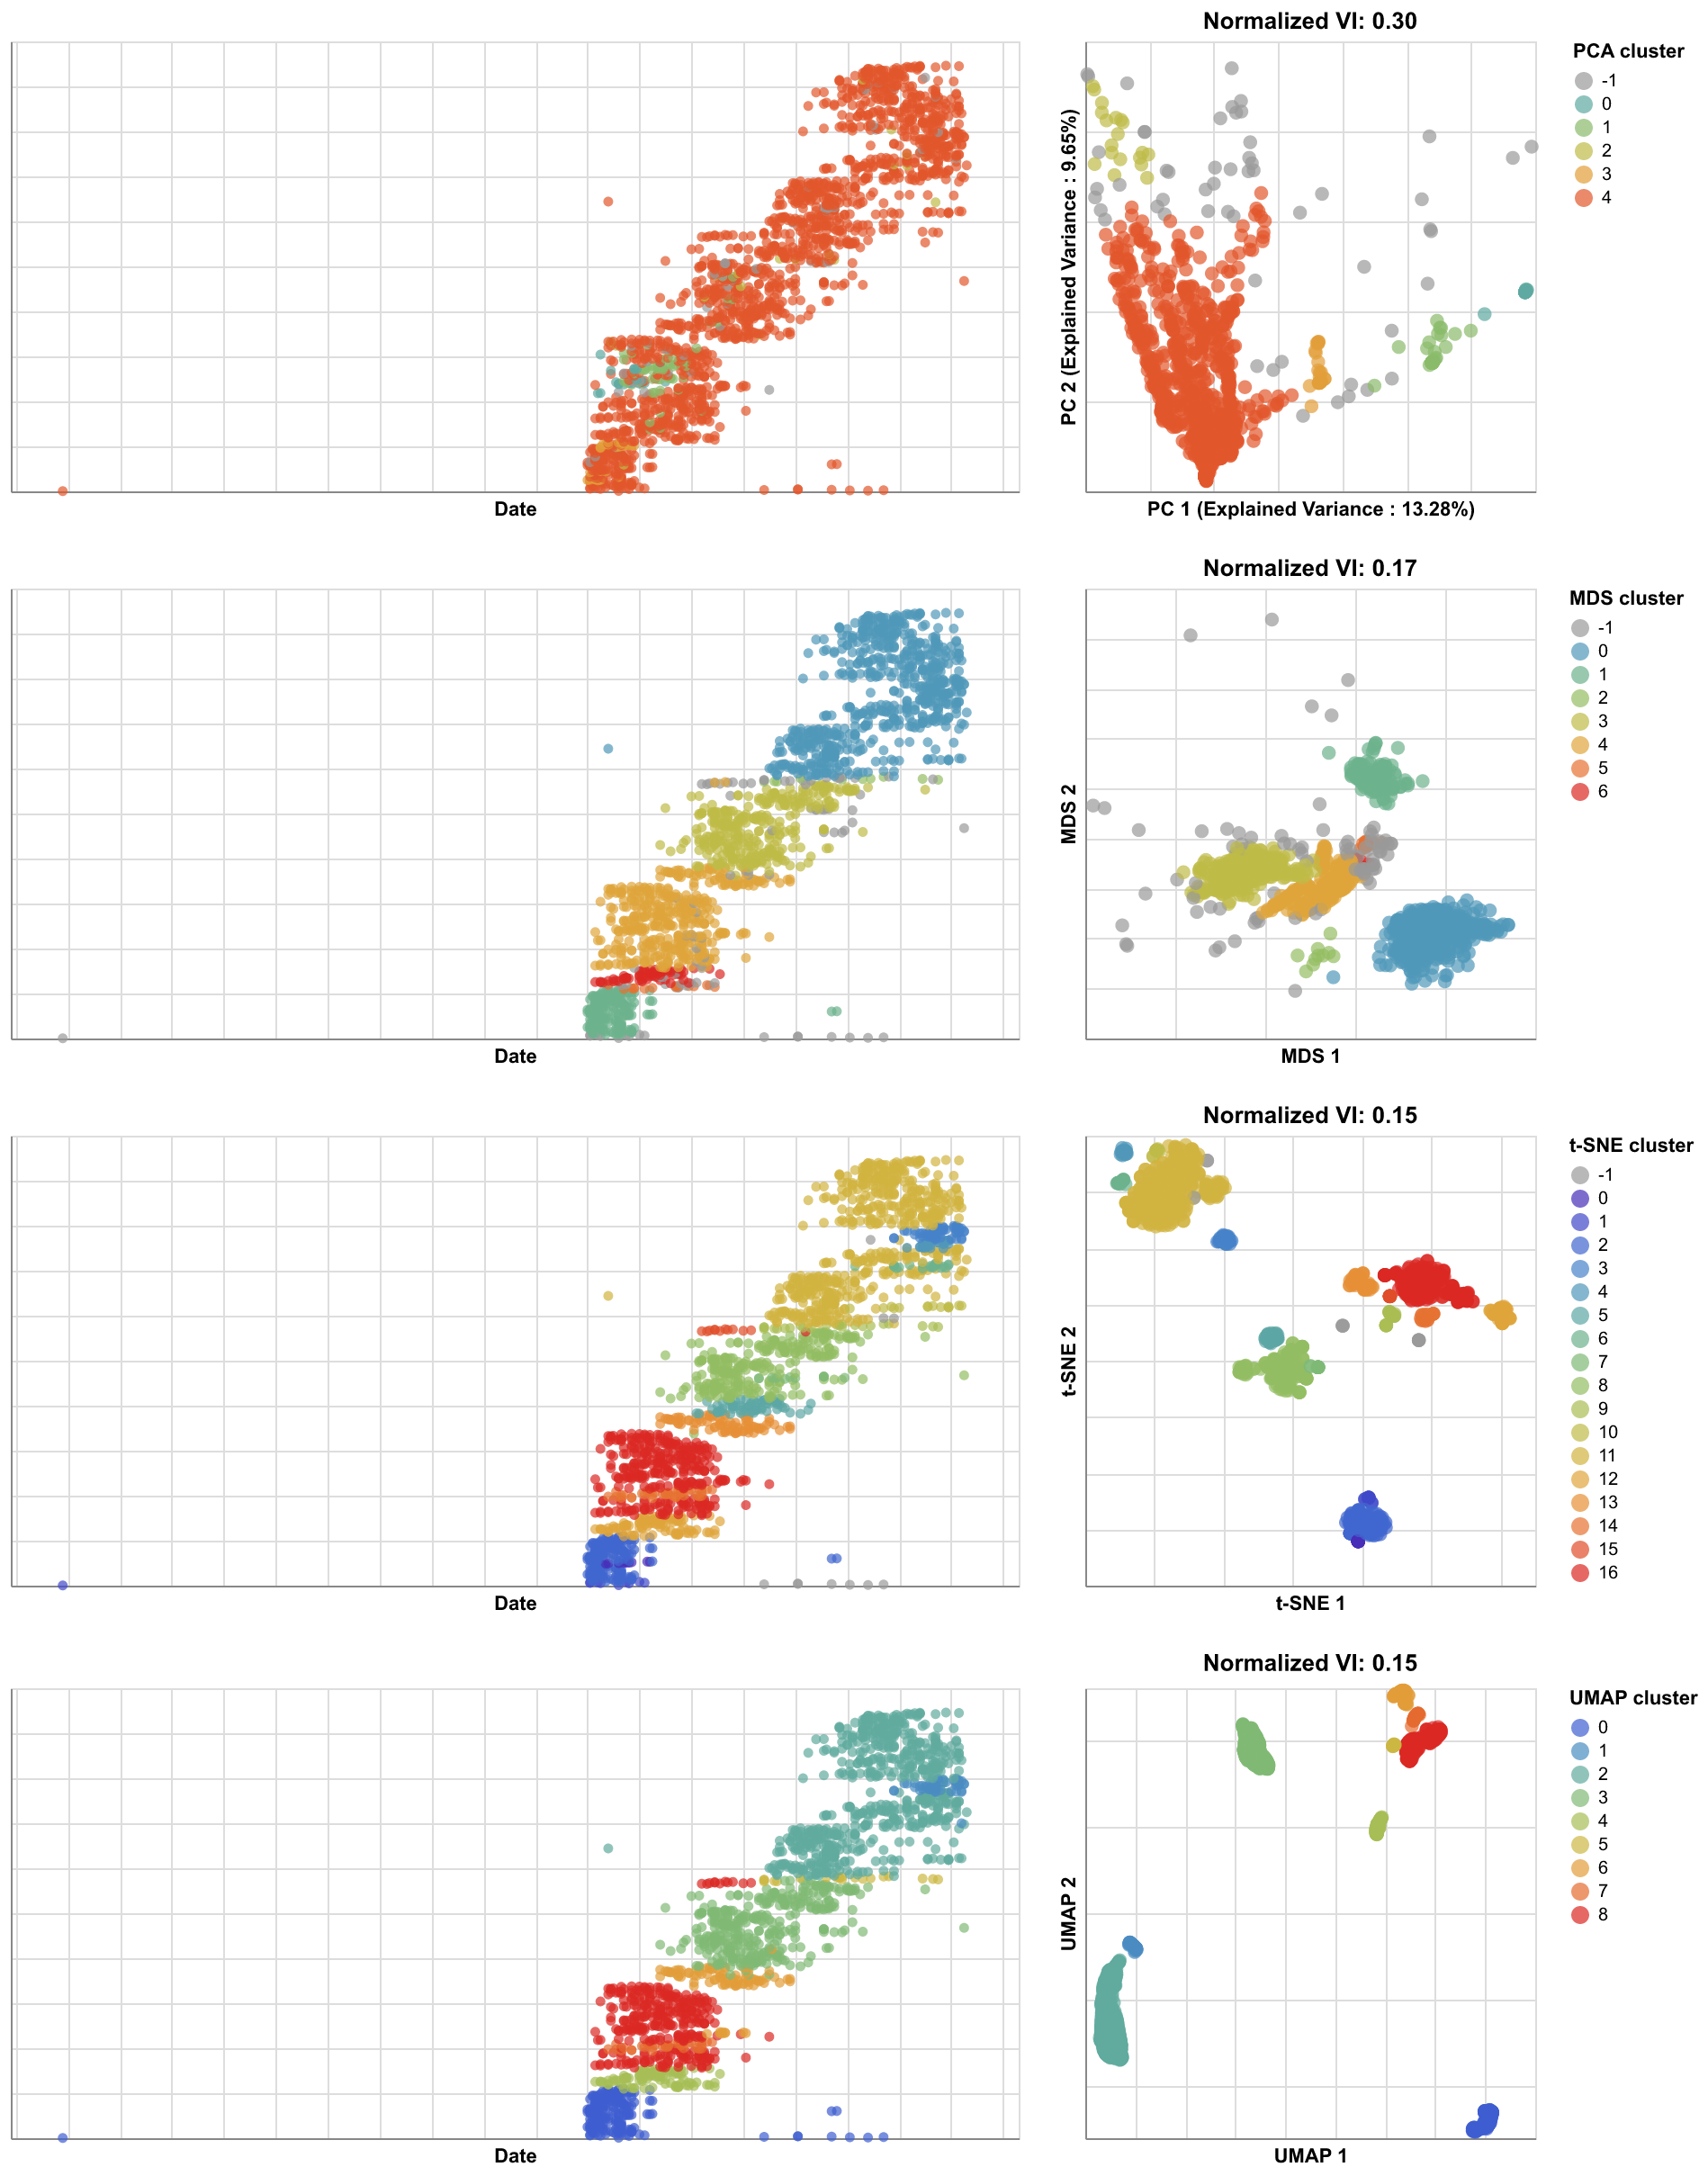
\includegraphics[width=\columnwidth]{figures/sarscov2-test-embeddings-by-cluster-vs-Nextstrain_clade.png}
\caption{{\bf Embeddings of SARS-CoV-2 sequences collected between January 1, 2022 and July 5, 2023 colored by embedding cluster and annotated by normalized VI to indicate accuracy of clusters for training data compared to expert clade assignment (Nextstrain clade).}
}
\label{fig:sars-cov-2-2022-2023-clusters-vs-Nextstrain-clade}
\end{figure}

\section*{Discussion}

TBD.

\section*{Conclusion}

TBD.

\section*{Supporting information}

% Include only the SI item label in the paragraph heading. Use the \nameref{label} command to cite SI items in the text.

\section*{Acknowledgments}
TBD.

\nolinenumbers

% Either type in your references using
% \begin{thebibliography}{}
% \bibitem{}
% Text
% \end{thebibliography}
%
% or
%
% Compile your BiBTeX database using our plos2015.bst
% style file and paste the contents of your .bbl file
% here. See http://journals.plos.org/plosone/s/latex for
% step-by-step instructions.
%

% TODO: copy/paste bbl file contents below instead of using standard bibliography commands.
\bibliographystyle{plos2015}
\bibliography{cartography}

% \begin{thebibliography}{10}

% \bibitem{bib1}
% Conant GC, Wolfe KH.
% \newblock {{T}urning a hobby into a job: how duplicated genes find new
%   functions}.
% \newblock Nat Rev Genet. 2008 Dec;9(12):938--950.

% \bibitem{bib2}
% Ohno S.
% \newblock Evolution by gene duplication.
% \newblock London: George Alien \& Unwin Ltd. Berlin, Heidelberg and New York:
%   Springer-Verlag.; 1970.

% \bibitem{bib3}
% Magwire MM, Bayer F, Webster CL, Cao C, Jiggins FM.
% \newblock {{S}uccessive increases in the resistance of {D}rosophila to viral
%   infection through a transposon insertion followed by a {D}uplication}.
% \newblock PLoS Genet. 2011 Oct;7(10):e1002337.

% \end{thebibliography}

\end{document}
